\documentclass{csse4400}

% \teachermodetrue

\usepackage{float}

\usepackage{languages}

\title{Scaling Stateless Components}
\author{Evan Hughes \& Anna Truffet \& Brae Webb }

\date{\week[practical]{6}}
\begin{document}

\maketitle

\begin{figure}[h]
    \begin{center}
        
\includegraphics[scale=0.4]{images/scaling-out}
    \end{center}
\end{figure}

\section{This Week}
Our goal is to scale out the stateless component of our TaskOverflow application across multiple compute instances.
Specifically we will need to:
\begin{itemize}
    \item Route traffic to our deployed TaskOverflow application with a load balancer.
    \item Scale out TaskOverflow instances with autoscaling.
    \item Check the status of our instances with a healthcheck.
    \item Dynamically scale our application based on load.
\end{itemize}

\section{Load Balancers}

Load balancing distributes a load over a set of resources.
For example, balacing network traffic across several servers.
Load balancing is crucial to the scalability of modern systems, as often, one physical device can not process the large amount network traffic for (e.g.) a large website.

A service which load balances, is called a \textbf{Load Balancer}.


\subsection{Routing Algorithms}

A load balancer can implement many techinques to select which resource to route incoming requests toward, these techniques are the load balancer's routing algorithm.

Below lists several common routing techniques.
There are many other generic and bespoke routing algorithms that are not listed.

\begin{description}
  \item[Round Robin] allocates requests to the next available server regardless of where the last request was sent.
      It is simple, and in practice, works effectively.
  \item[Least Connections] sends the next request to the node with the fewest current connections.
      The load balancer is responsible for tracking how many connections exist to each node.
  \item[Weighted Least Connections] sends the next request to the node with the least weighted connections. This is similar to the above least connections method, however, each node has an associated weight.
      This allows certain nodes to be preferred over others.
      This is useful if we have an inequal distribution of compute power.
      We would want to give smaller nodes a reduced load in comparison to other more powerful nodes.
  \item[Consistent Hashing] In some cases we may want a user to consistently be routed to a specific node.
      This is useful for multiple transactions that need to be done in a consistent order or if the data is stored/cached on the node.
      This can be done by hashing the information in the request payload or headers and then routing the request to the node that handles hashes in the range of the computed hash.
\end{description}

\subsection{Health Checks}

When load balancing, it is important to ensure that the nodes we route requests to are able to service the request.
A good health check can save or break your service.
Consider the two following examples from UQ's Information Technology Services (ITS):

\paragraph{Example 1} Early in my career, I, Evan Hughes, setup a multi-node Directory Server at UQ under the hostname of \texttt{ldap.uq.edu.au}.
This server was a NoSQL database which implemented the LDAP protocol and supported \texttt{UQ Authenticate},
UQ's Single Sign-On service.

The service had a load balancer which checked that \texttt{port 389} is open and reachable. 
This worked well most of the time.
However, the health check was too weak. When:
\begin{enumerate} 
    \item A data-center outage occured; and
    \item The operating system running the service disappeared; but 
    \item The service was still running in memory.
\end{enumerate}

The health check passed, but in reality, the service was talking to dead nodes, causing upstream services to have intermitent failures. 

\todo{C4 Diagram of the architecture}

\paragraph{Example 2} During the rollout of a new prompt for UQ Authenticate which required users to go to my.UQ to provide verified contact details - the Blackboard (learn.uq.edu.au) service went completly offline.
The health check for Blackboard at the time completed a full authentication as a test user to ensure everything was functioning as expected.
Once this user was enrolled into the new rollout,
the health checks started reporting failures and within a matter of minutes the entire pool of nodes were shutdown.
This health check was too broad and was not isolated enough to the service that it was checking.

\todo{C4 diagram of the architecture}

A lot of services will provide a health check endpoint or a metrics endpoint which can help the engineer setup a proper level of health check.
We want a health check that is specific enough for the service that it is checking but not so specific that it is too brittle.
For the TaskOverflow application that we have been building so far,
a reasonable health check would be that the health endpoint ensures the database is available and that the application is able to connect to it.

\section{Load Balancers in AWS}

\subsection{Types of AWS Load Balancers}
Not all load balancers are the same.
Some load balancers inspect the transmitted packets to correctly route the packet.
We will cover two load balancer types AWS provides:

\begin{description}
  \item[Application Load Balancer] is an OSI layer 7%
\footnote{OSI layer 7: Application, in this case HTTP/HTTPS/etc}
load balancer which routes traffic based on the request's content.
      This is useful for services using HTTP, HTTPS, or any other supported protocol.
  \item[Network Load Balancer] is an OSI layer 4%
\footnote{OSI layer 4: Transport, in this case TCP/UDP}
load balancer which routes traffic based on the source and destination IP addresses and ports.
This is useful for services that are using TCP or UDP.
\end{description}

\subsection{AWS Load Balancer Design}

An AWS Elastic Load Balancer has three distinct components. 

\begin{description}
  \item[Listeners] allows traffic to enter the Elastic Load Balancer.
  Each listener has a port (e.g. \texttt{port 80}) and a protocol (e.g. \texttt{HTTP}) associated with it.
  \item[Target Groups] are groups of nodes which the load balancer can route to. 
      Each target group has a protocol and a port associated with it, allowing us (the programmer) to switch ports on the way through the load balancer.
      This is useful if the targets are using a different port to the ports we want to expose.
  \item[Load Balancer] is the actual load balancer that routes the traffic to the target groups based on rules that we setup.
      The load balancer has a DNS name that we can use to route traffic to it.
      The load balancer also has a security group that we can use to control what traffic can enter the load balancer. 
\end{description}

\begin{figure}[H]
  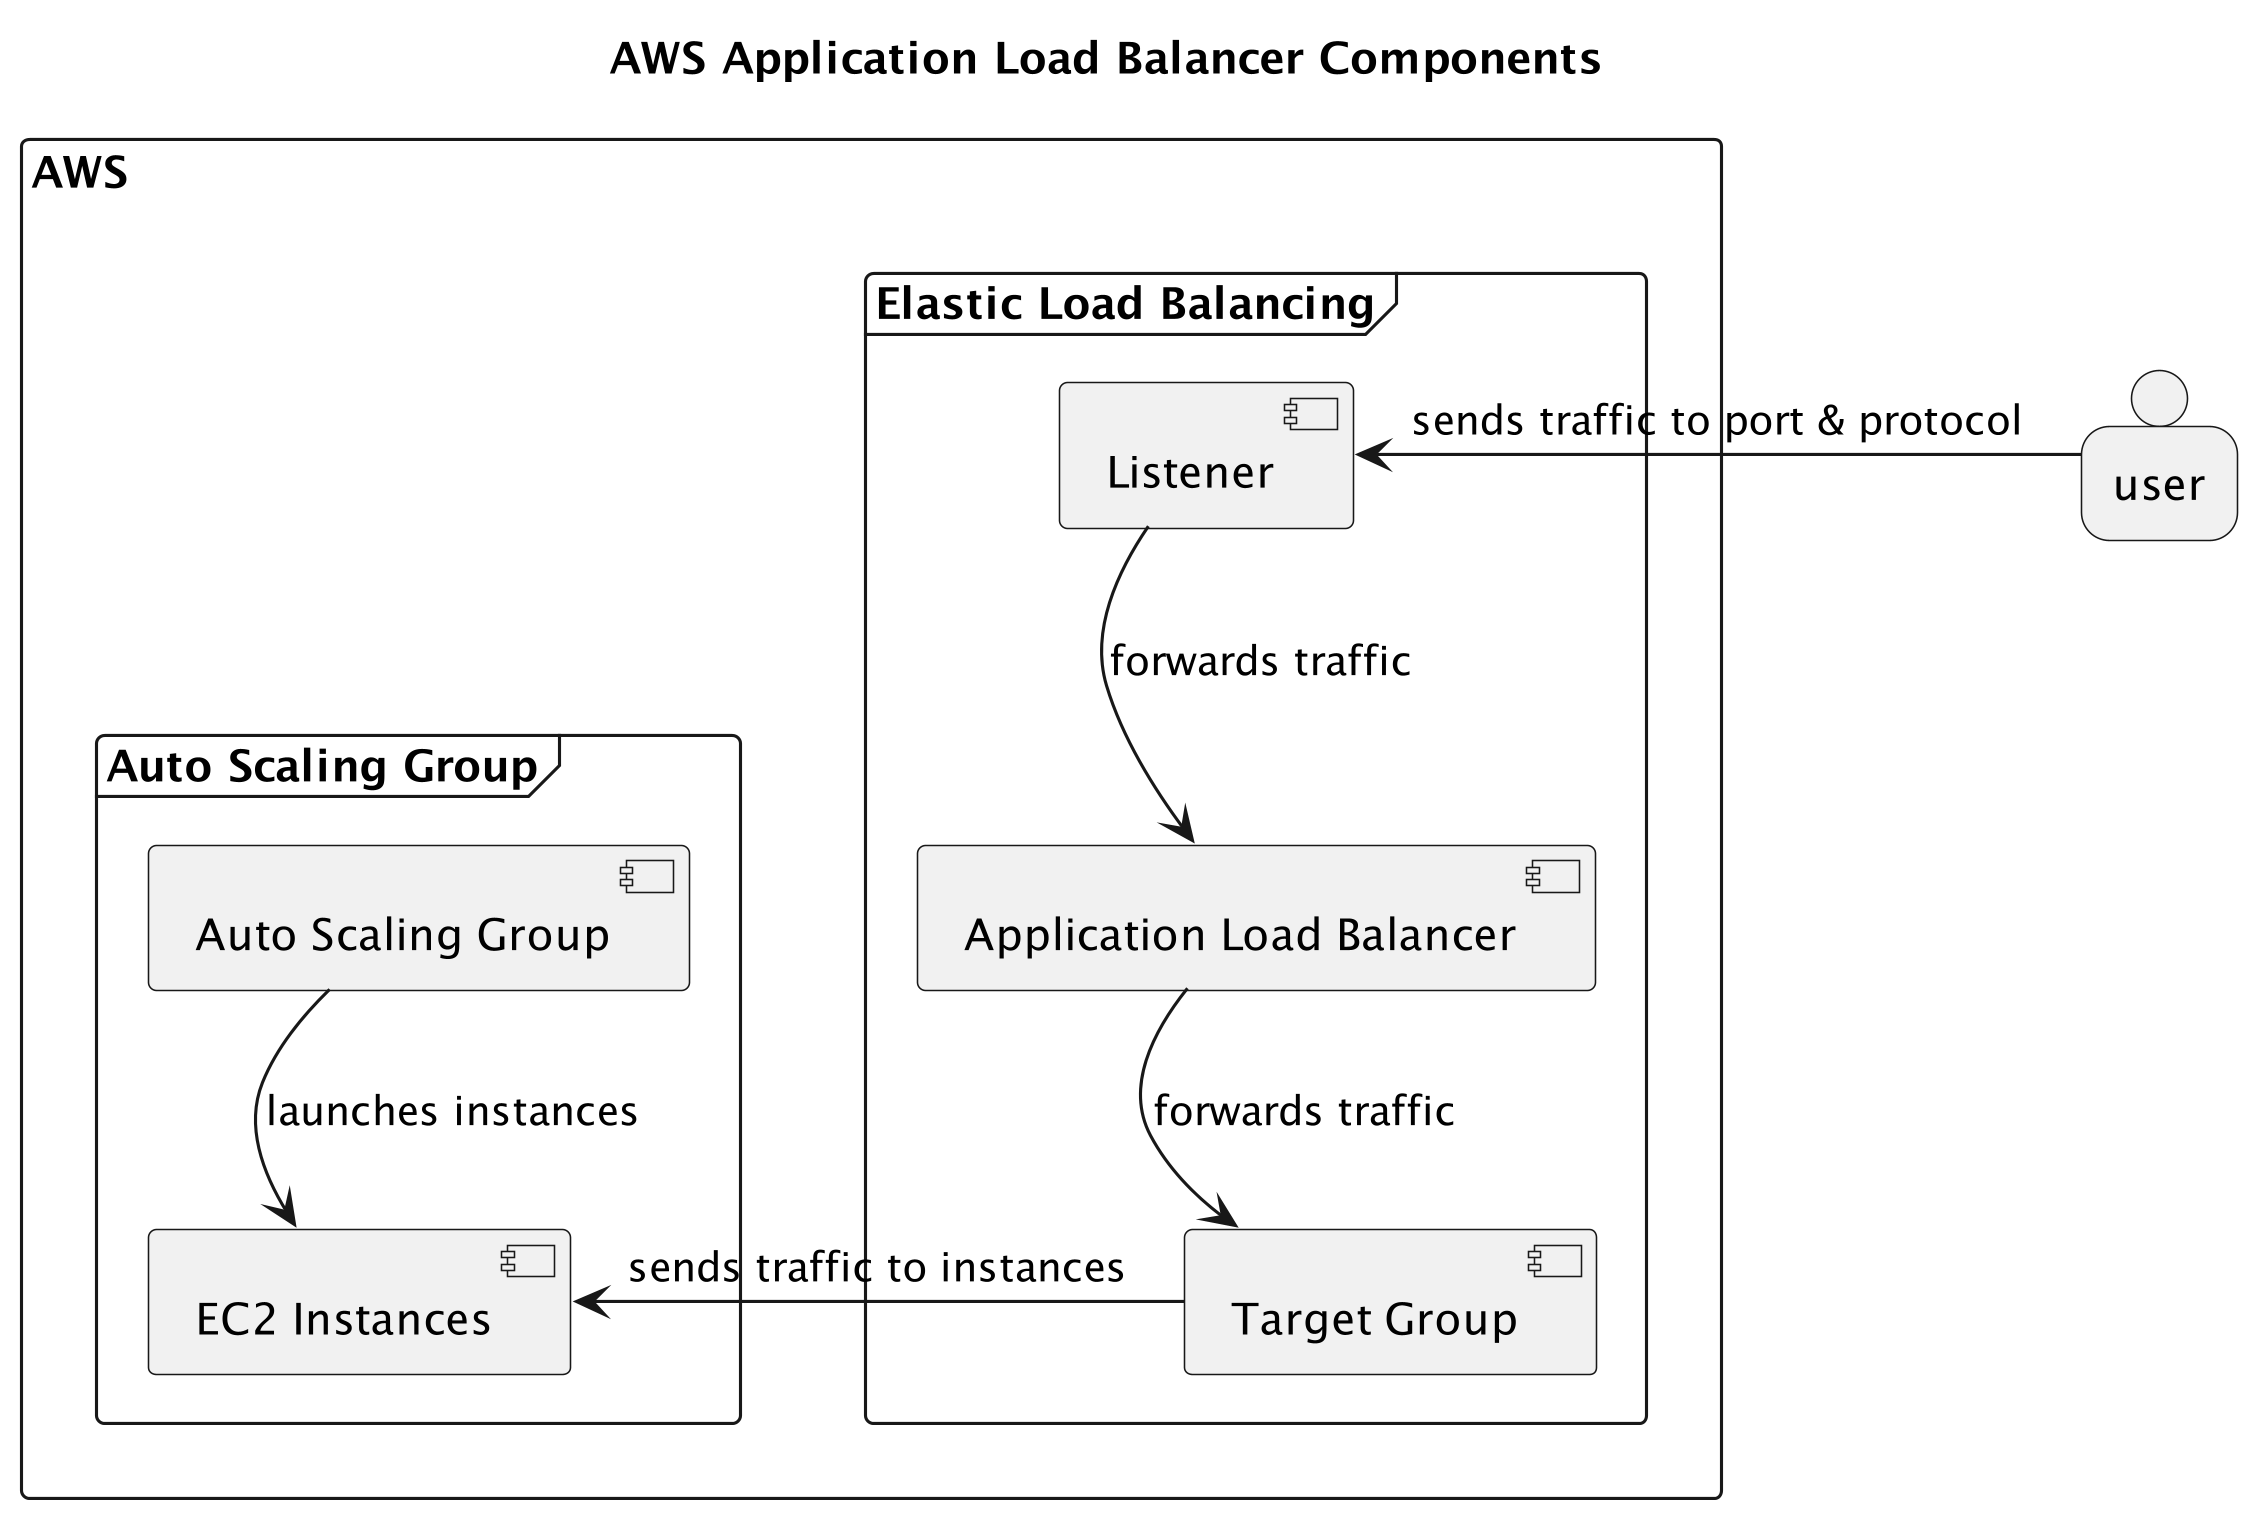
\includegraphics[width=\textwidth]{diagrams/loadbalancers}
\end{figure}

\subsection{Autoscaling in AWS}
Instead of creating the maxiumum amount of services we predict we will need,
we can automatically scale the number of nodes we need to minimise resources.
When the load is low, we operate with minimal nodes.
When the load is high, we increase the number of nodes available to cope.

To compute the resources needed, AWS relies on triggers from CloudWatch and scaling policies.
Some premade triggers are based around a node's;

\begin{itemize}
    \item CPU usage,
    \item memory usage, or 
    \item network usage.
\end{itemize}

We create custom triggers based on our application's metrics.

\section{Load Balancing TaskOverflow}

This week we are going to explore load balancing the TaskOverflow service that we have been working with. The aim is to have a service that when given a lot of requesters will be able to scale out the webservice nodes to handle it. This wont be a full solution to the scaling issue as our database is still a single node, but it will be a good start. Other methods could also be employed to help deal with the load like caching but we will leave that for another day.

Start with the github repository provided in class and install terraform as it will be required this week. You will also need to start your learner lab and copy the credentials into a credentials file into the root of the respository. In the respository you will also see two differnt folders, one is the starter for the EC2 path and the other is the starter for the ECS path. Once you have chosen which path you want to take, copy the contents of the folder into the root of the repository.

As per last week, we encourage that you take \texttt{Path B} first and then pruse the \texttt{Path A} if you have time. This week \texttt{Path A} does show an alternative method to autoscaling.

\subsection{[Path A] EC2}

Congratulations! You have chosen to go down the EC2 path, this week we need to create a AutoScaling Group and a Load Balancer to handle the scaling of our service. Our goal is the deployment diagram below.

\begin{figure}[H]
  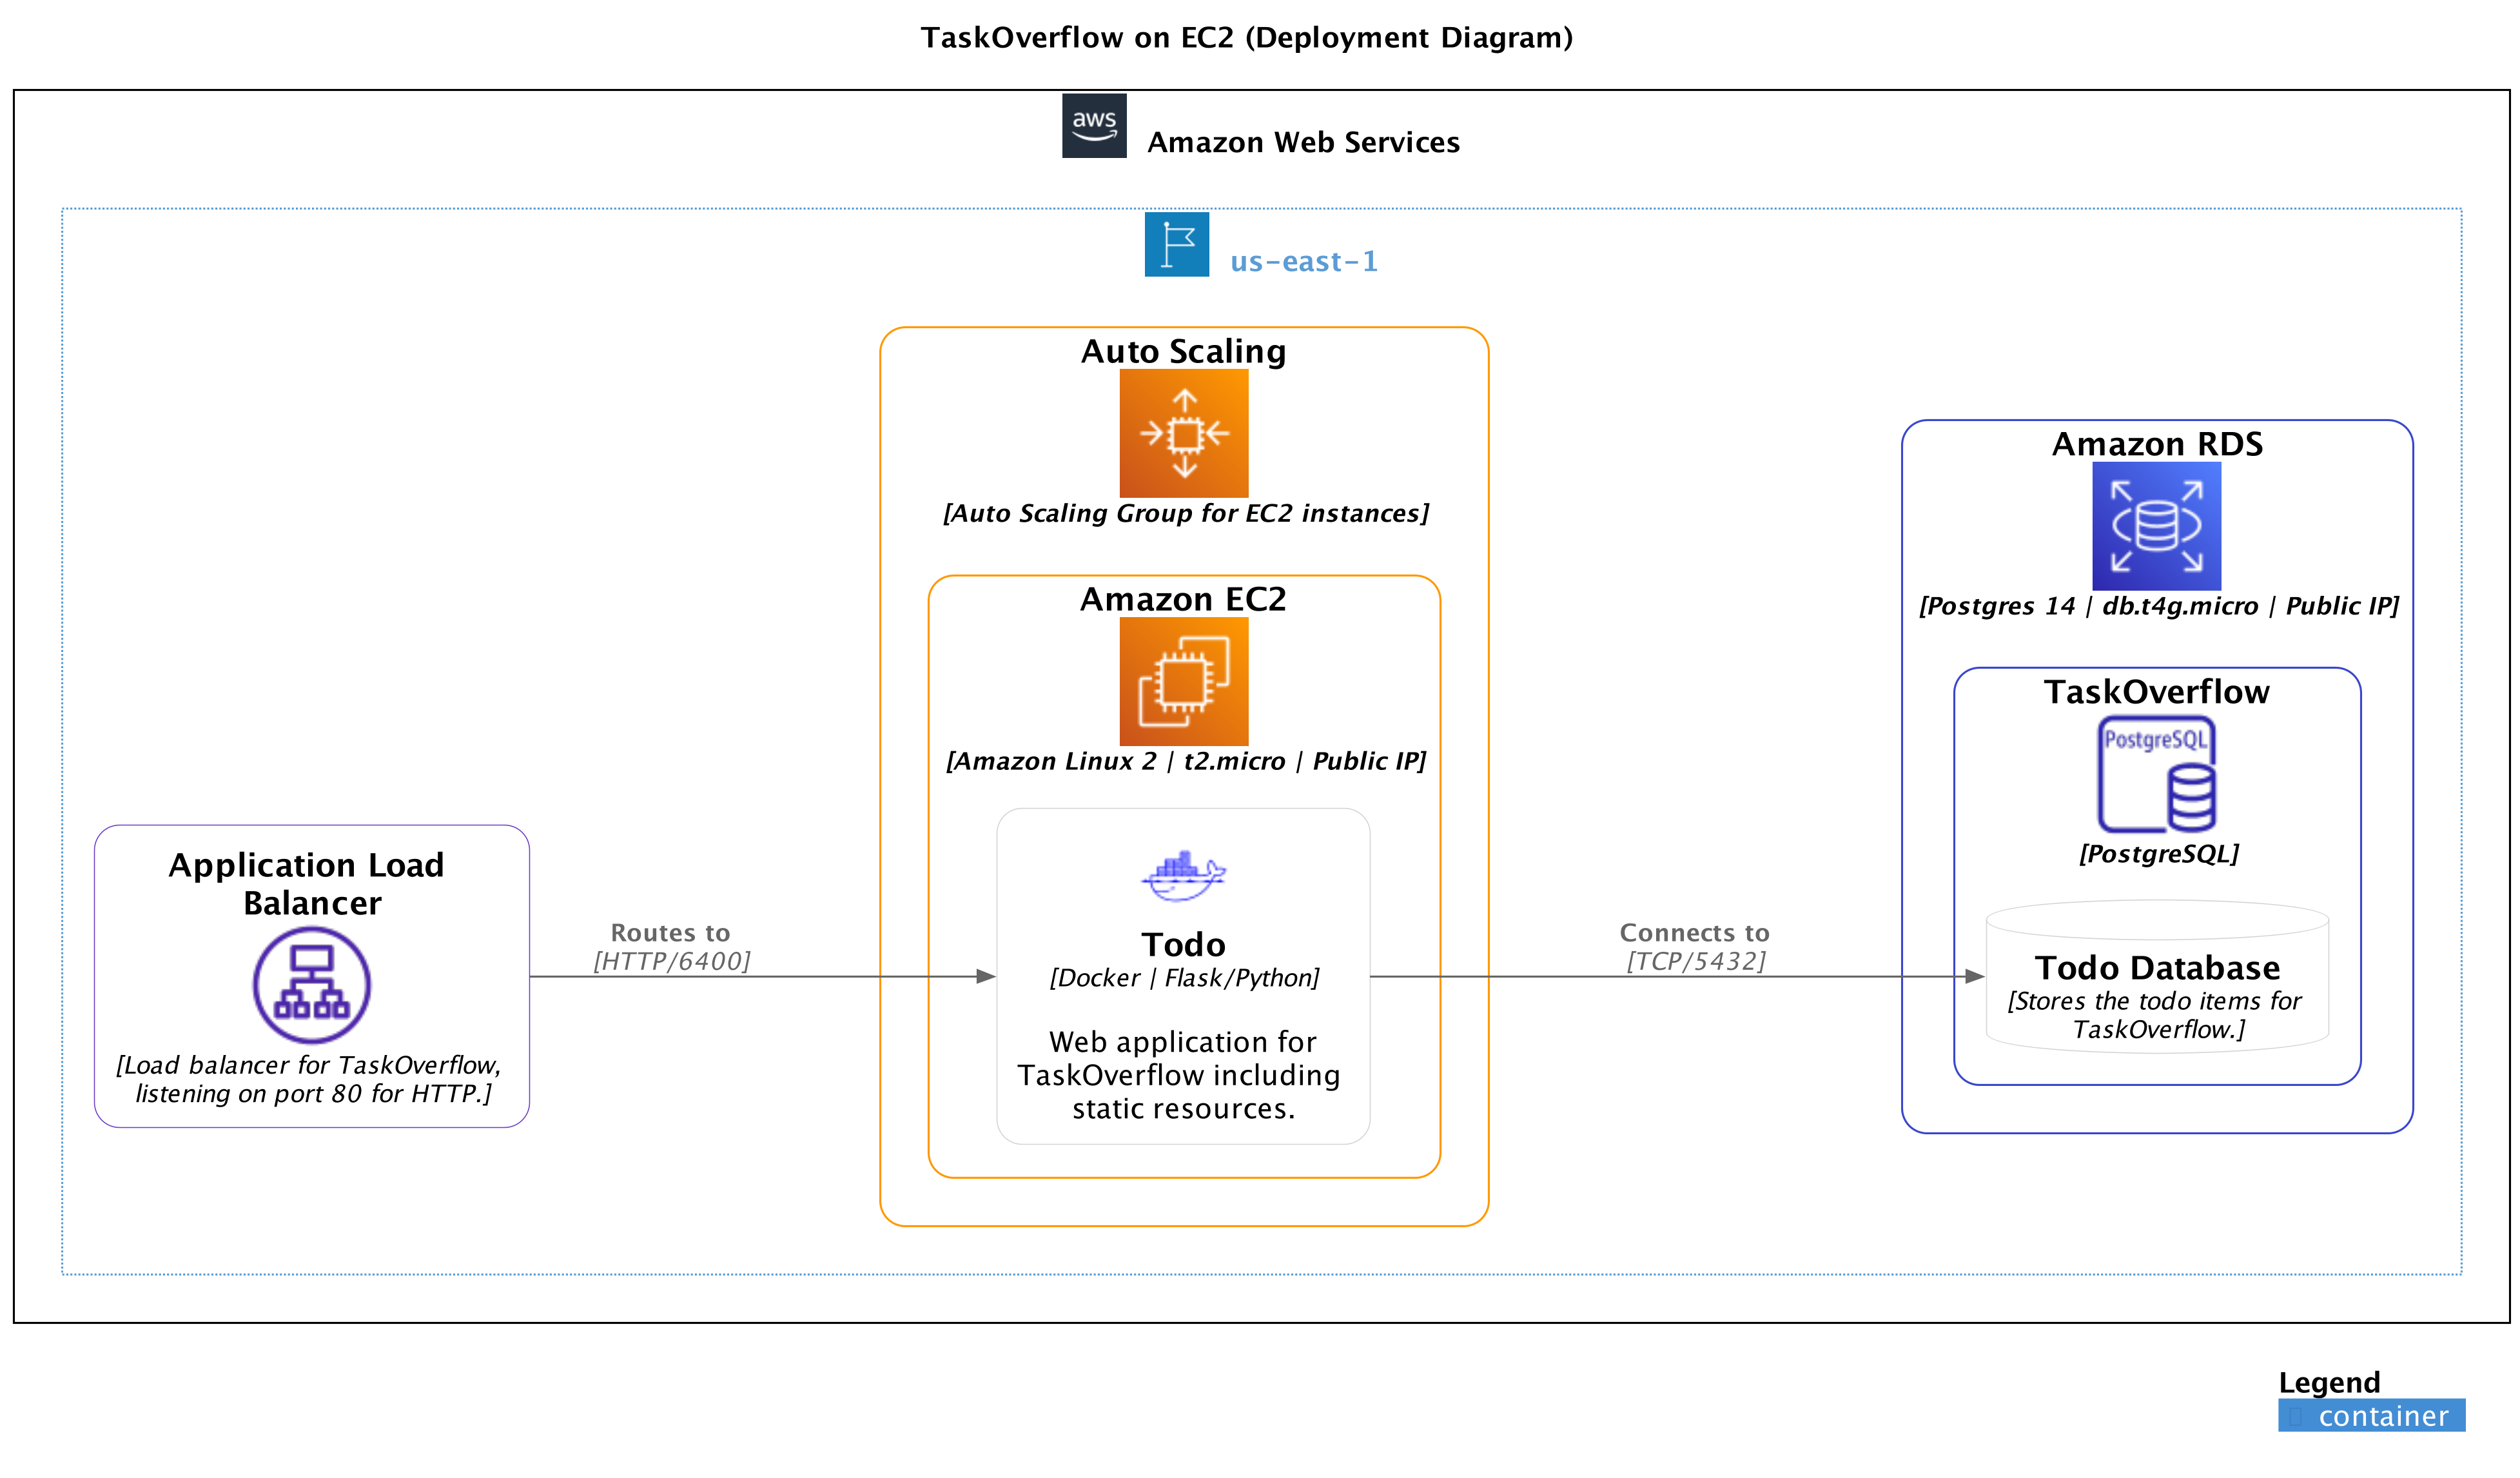
\includegraphics[width=\textwidth]{diagrams/ec2deployment}
\end{figure}

To get started we need to modify how we create our EC2 instances, instead of manually creating them we are going to have to teach AWS how to deploy them for us. We can do this by converting our EC2 instance into a Launch Template. Our launch template is going to look very similar to the instance we had last week, instead a few variables have changed including that our user\_data must be stored as a base64 encoded string. Some of these changes have been highlighted below, also copy this code into a file called \texttt{ec2.tf}.


\begin{code}[language=terraform,numbers=none,escapechar=|,keepspaces=true]{ec2.tf}
resource "aws_launch_template" "todo" {
  name          = "todo-launch-template"
  |\colorbox{yellow}{image\_id}|     = "ami-005f9685cb30f234b"
  instance_type = "t2.micro"
  key_name      = "vockey"
  user_data     = |\colorbox{yellow}{base64encode}|(<<-EOT
    #!/bin/bash
    yum update -y
    yum install -y docker
    service docker start
    systemctl enable docker
    usermod -a -G docker ec2-user 
    docker run --restart always -e SQLALCHEMY_DATABASE_URI=postgresql://${local.database_username}:${local.database_password}@${aws_db_instance.database.address}:5432/todo -p 6400:6400 ${local.image}
EOT
  )

  vpc_security_group_ids = [aws_security_group.todo.id]
}


resource "aws_security_group" "todo" {
  name          = "todo"
  description   = "TaskOverflow Security Group"

  ingress {
    from_port   = 6400
    to_port     = 6400
    protocol    = "tcp"
    cidr_blocks = ["0.0.0.0/0"]
  }

  ingress {
    from_port   = 22
    to_port     = 22
    protocol    = "tcp"
    cidr_blocks = ["0.0.0.0/0"]
  }

  egress {
    from_port   = 0
    to_port     = 0
    protocol    = "-1"
    cidr_blocks = ["0.0.0.0/0"]
  }
}
\end{code}

Now that we have a template and a security group, we can create the AutoScaling Group. This block defines the limits of how many instances we want to have and the template we want it to use. Copy this code into a file called \texttt{autoscaling.tf}.

\begin{figure}[H]
  \begin{center}
    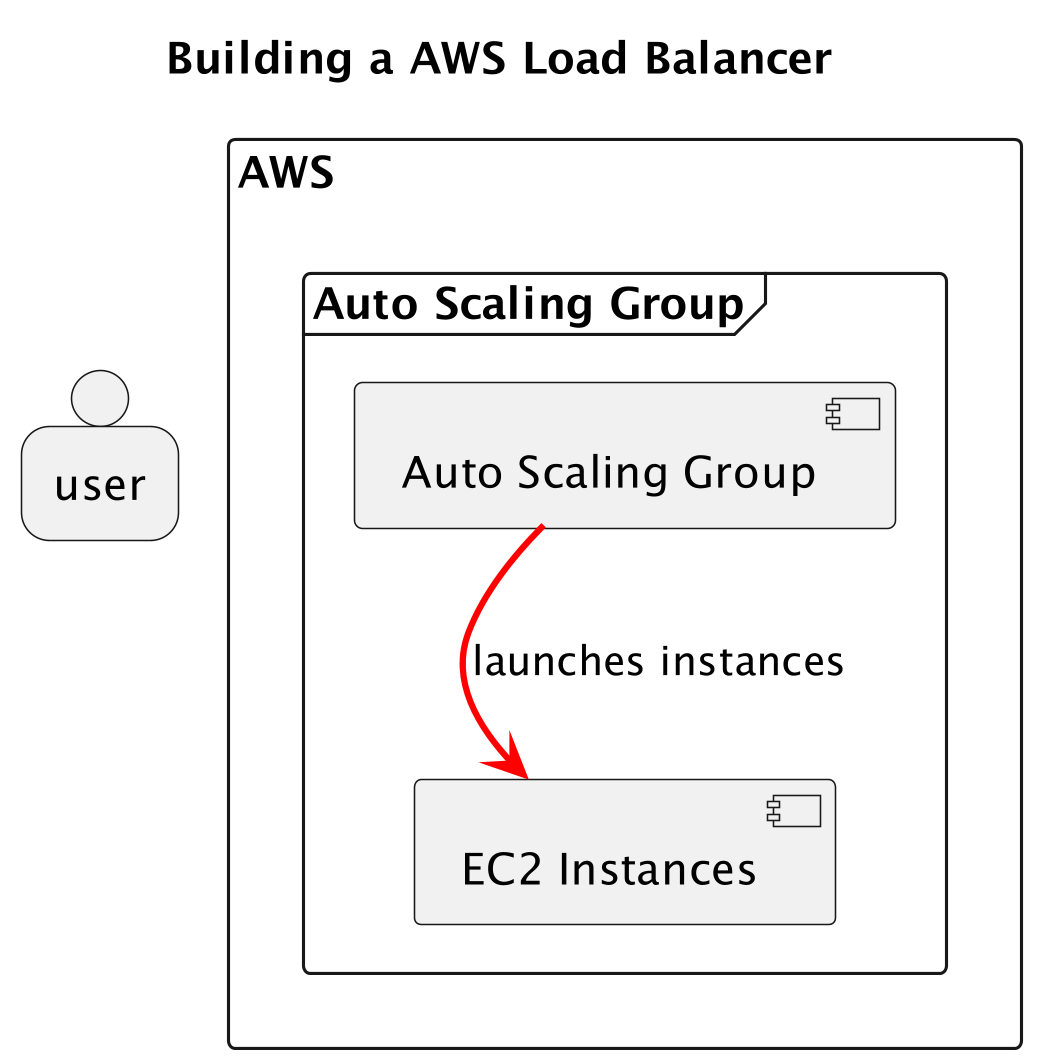
\includegraphics[scale=0.2]{diagrams/lb1}
  \end{center}
\end{figure}

\begin{code}[language=terraform,numbers=none,keepspaces=true]{autoscaling.tf}
resource "aws_autoscaling_group" "todo" {
  name               = "todo"
  availability_zones = ["us-east-1a"]
  desired_capacity   = 1
  max_size           = 4
  min_size           = 1
  
  launch_template {
    id      = aws_launch_template.todo.id
    version = "$Latest"
  }
}
\end{code}

If we deployed this now we would see that we get one initial instance created for us due to the desired and min\_size. Now that we have instances we have the ability for traffic to be routed to them. Lets create a target\_group which will be on the internal facing side of our load balancer. This is the side that lets traffic leave the load balancer and hit the instances. Copy this code into a file called \texttt{lb.tf}.

\begin{figure}[H]
  \begin{center}
    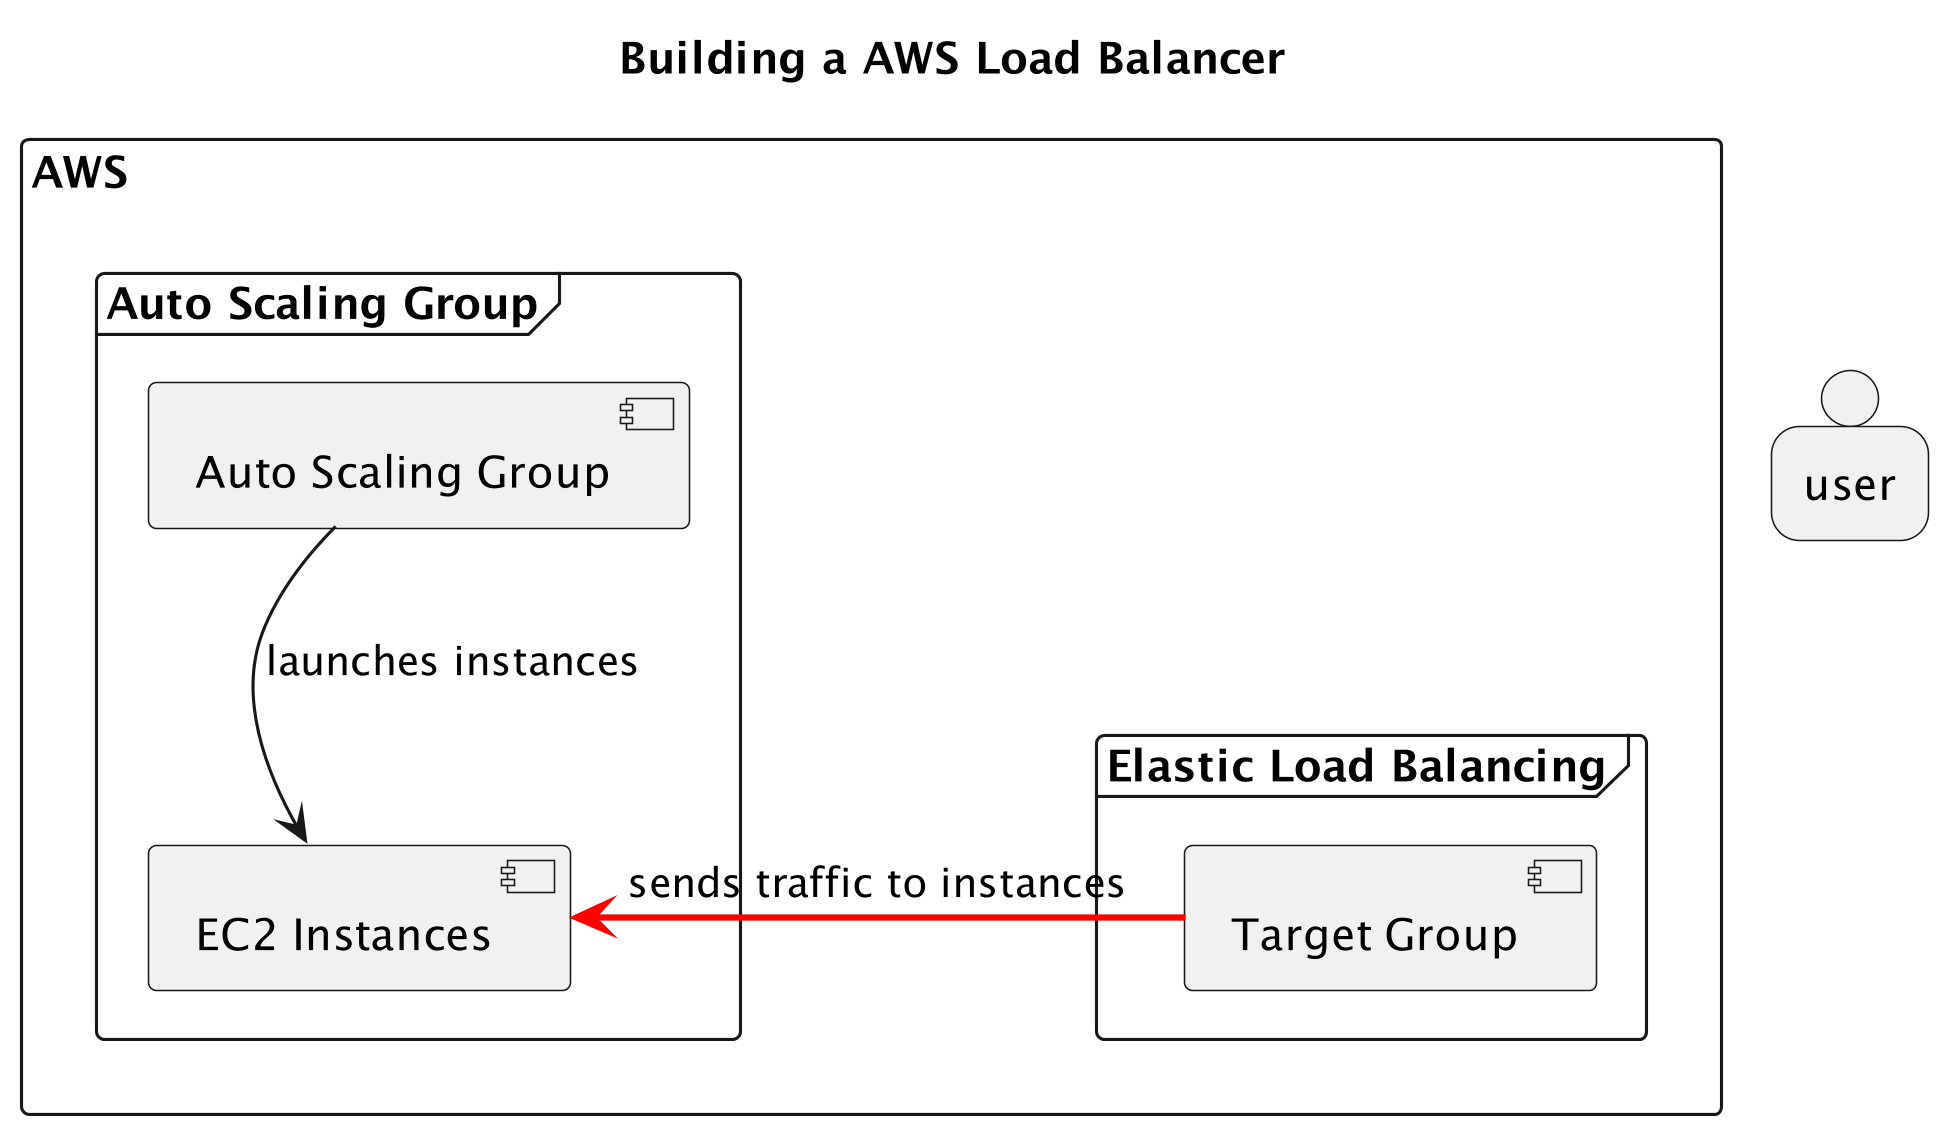
\includegraphics[scale=0.2]{diagrams/lb2}
  \end{center}
\end{figure}

\begin{code}[language=terraform,numbers=none,keepspaces=true]{lb.tf}
resource "aws_lb_target_group" "todo" {
  name     = "todo"
  port     = 6400
  protocol = "HTTP"
  vpc_id   = aws_security_group.todo.vpc_id
}
\end{code}

When the target\_group is created we need to attach it to the autoscaling group. This is done by via the code below, copy this into \texttt{lb.tf}.

\begin{code}[language=terraform,numbers=none,keepspaces=true]{lb.tf}
resource "aws_autoscaling_attachment" "todo" {
  autoscaling_group_name = aws_autoscaling_group.todo.id
  alb_target_group_arn   = aws_lb_target_group.todo.arn
}
\end{code}

With a target\_group made we now need to attach that to a load balancer, copy this code into \texttt{lb.tf}. You will notice that there is also a security group attached to the load balancer, this is the firewall that sits on the front of the load balancer and allows traffic to enter the load balancer.

\begin{figure}[H]
  \begin{center}
    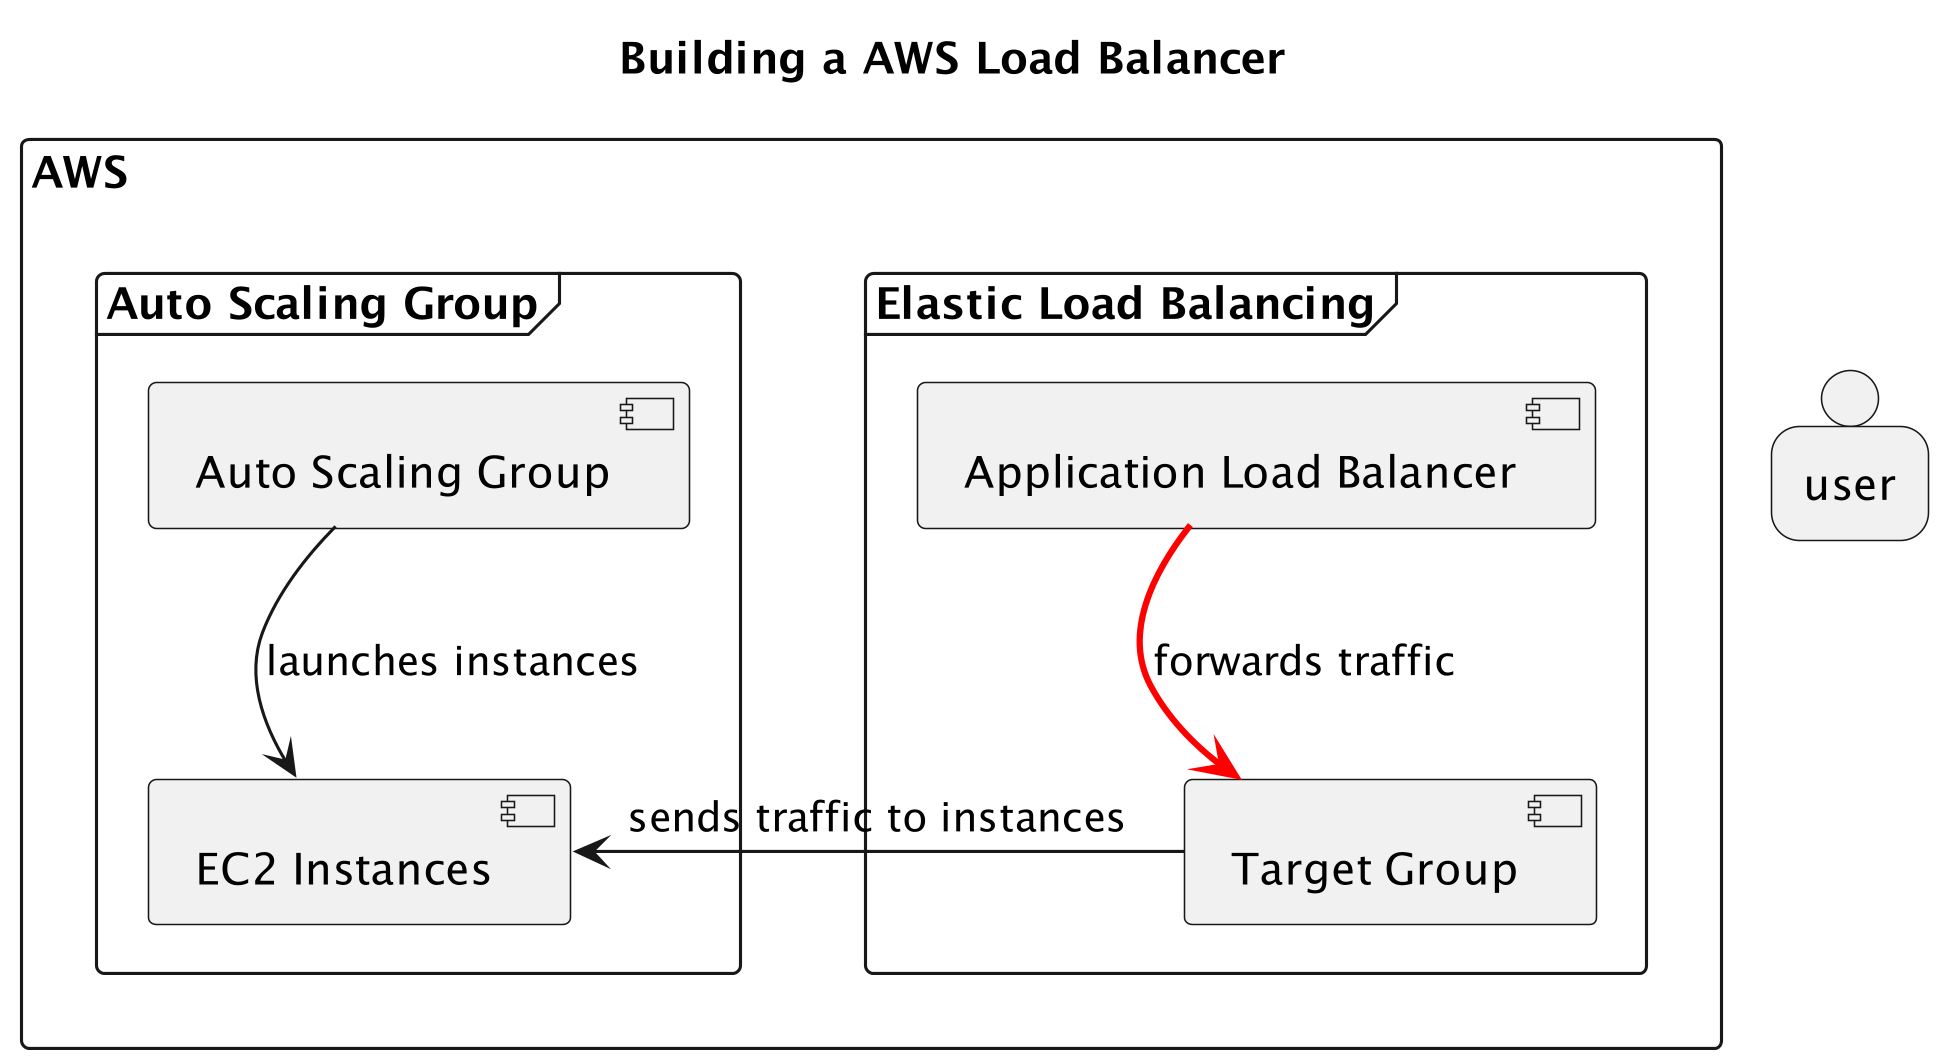
\includegraphics[scale=0.2]{diagrams/lb3}
  \end{center}
\end{figure}

\begin{code}[language=terraform,numbers=none,keepspaces=true]{lb.tf}
resource "aws_lb" "taskoverflow" {
  name               = "taskoverflow"
  internal           = false
  load_balancer_type = "application"
  subnets            = data.aws_subnets.private.ids
  security_groups    = [aws_security_group.taskoverflow.id]
}

resource "aws_security_group" "taskoverflow" {
  name          = "taskoverflow"
  description   = "TaskOverflow Security Group"

  ingress {
    from_port   = 80
    to_port     = 80
    protocol    = "tcp"
    cidr_blocks = ["0.0.0.0/0"]
  }

  egress {
    from_port   = 0
    to_port     = 0
    protocol    = "-1"
    cidr_blocks = ["0.0.0.0/0"]
  }
}
\end{code}

Now we are on the external side of the load balancer we need to create a listener which actually creates the rules for how traffic is routed to the instances. Copy this code into \texttt{lb.tf}.

\begin{figure}[H]
  \begin{center}
    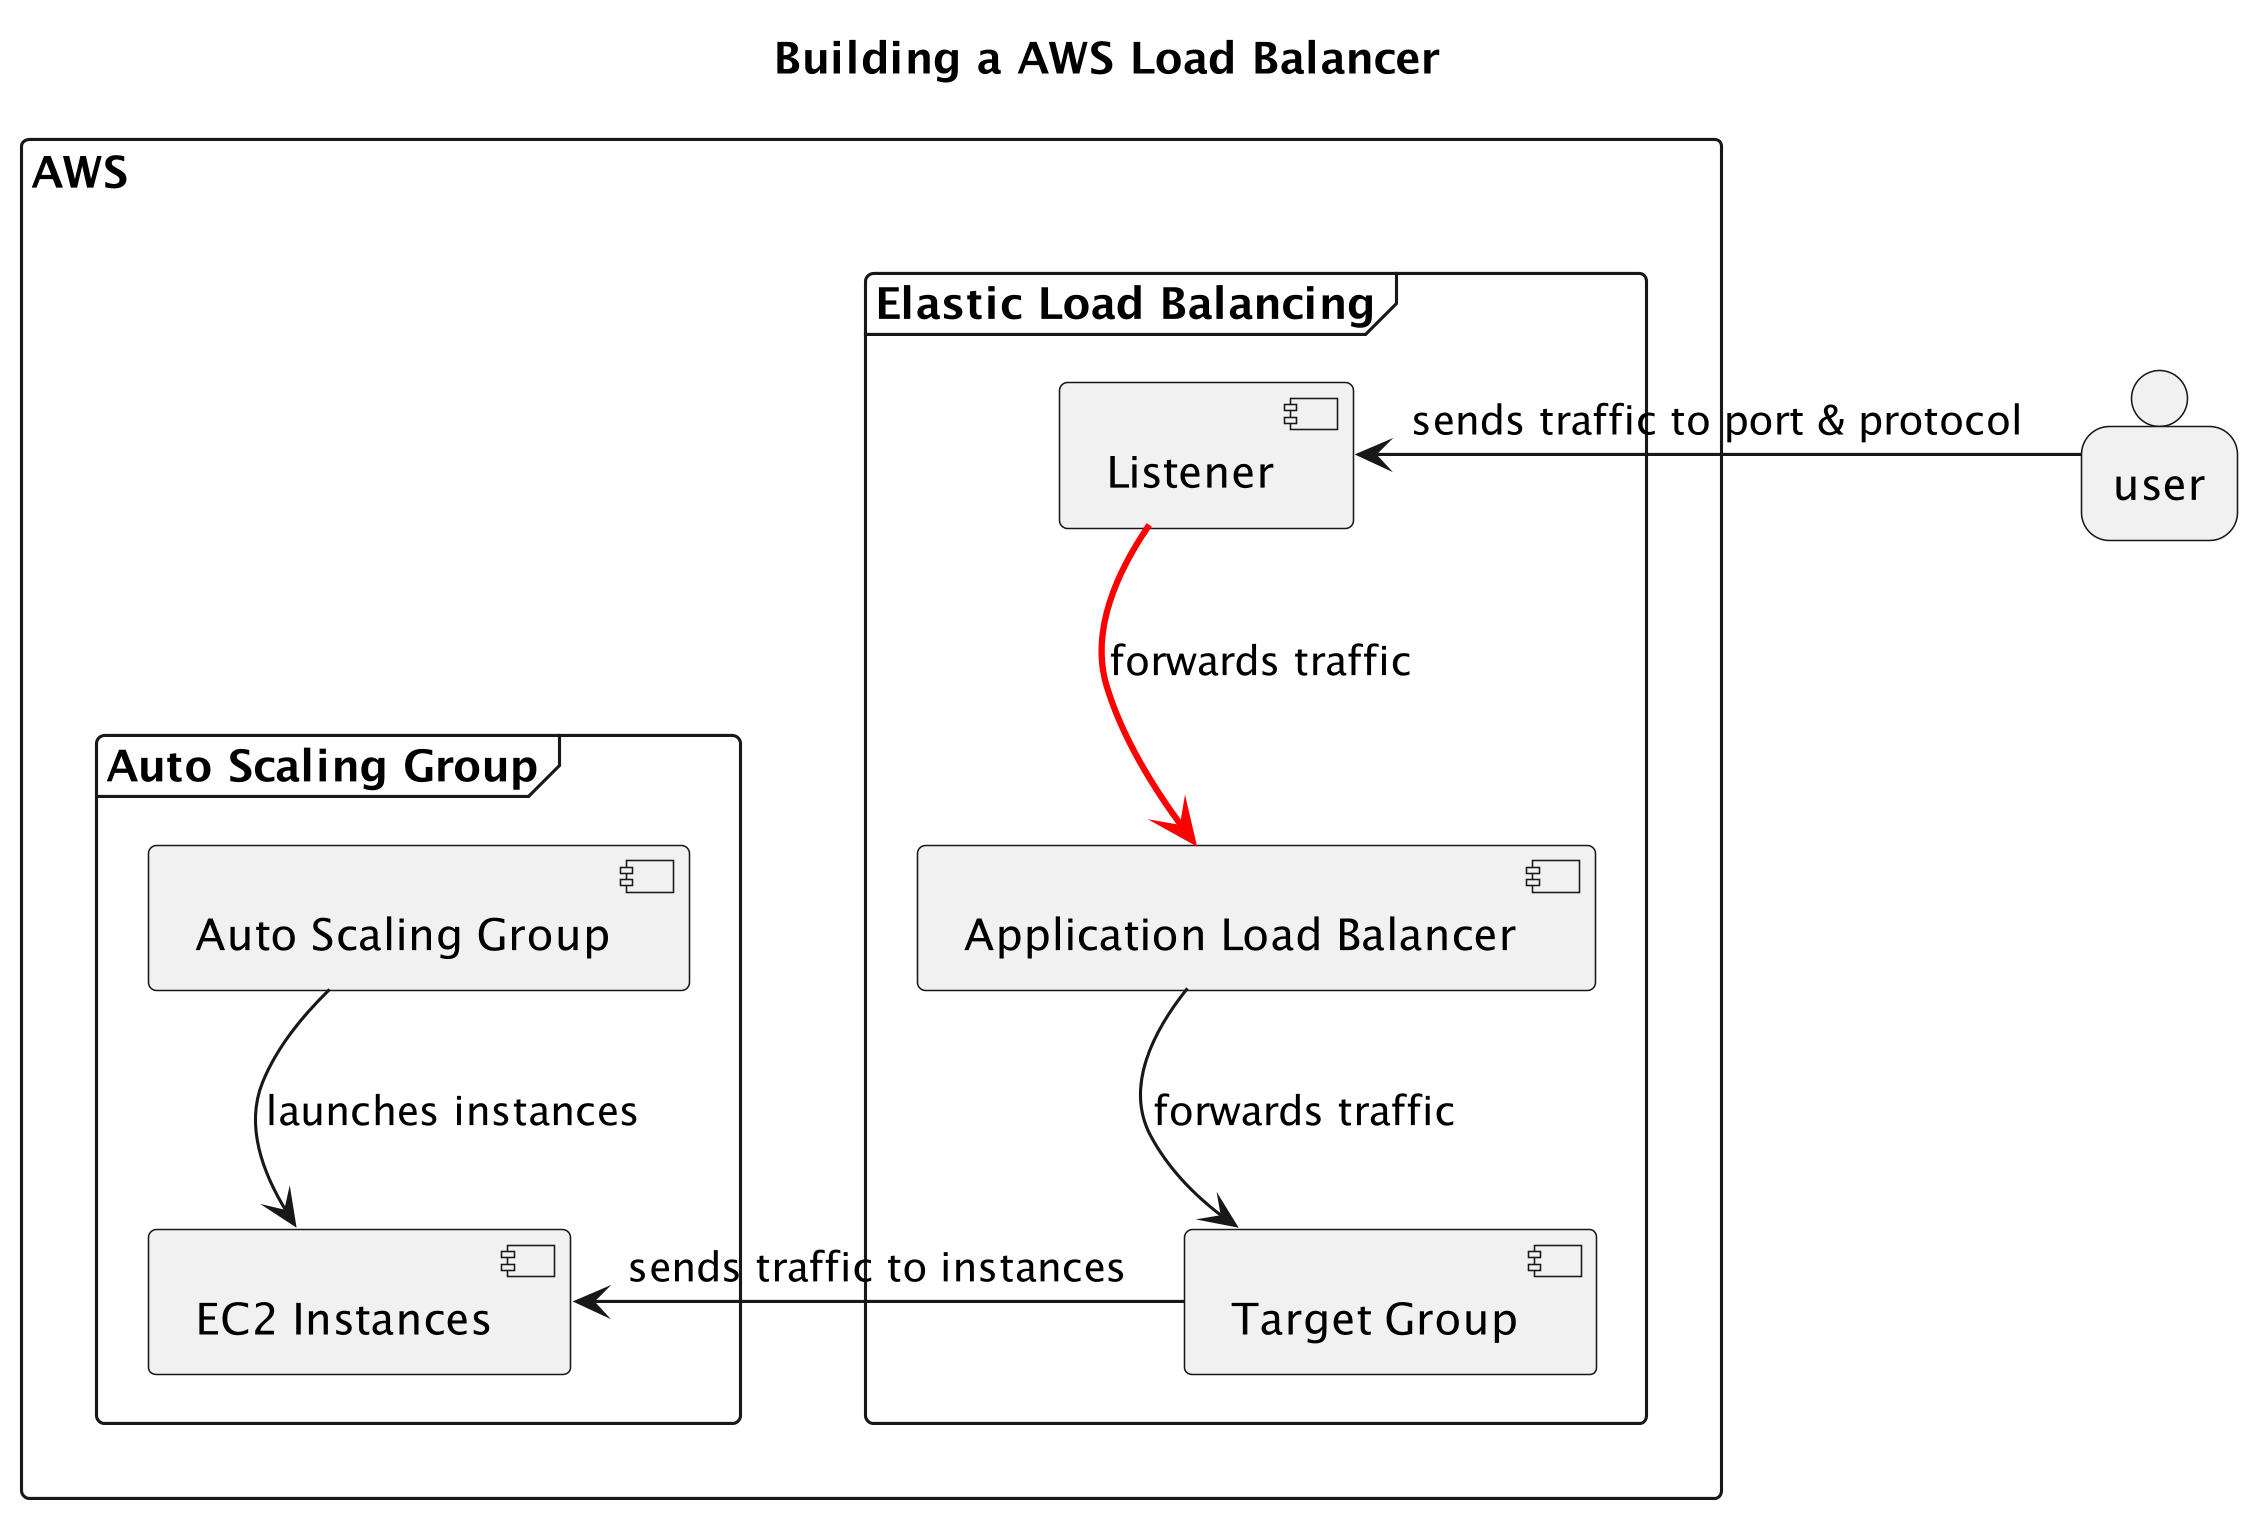
\includegraphics[scale=0.2]{diagrams/lb4}
  \end{center}
\end{figure}

\begin{code}[language=terraform,numbers=none,keepspaces=true]{lb.tf}
resource "aws_lb_listener" "taskoverflow" {
  load_balancer_arn = aws_lb.taskoverflow.arn
  port              = "80"
  protocol          = "HTTP"

  default_action {
    type             = "forward"
    target_group_arn = aws_lb_target_group.todo.arn
  }
}
\end{code}

Deploying this we now have achieved the architecture as requested with a dynamically scaling group of EC2s with a Application Load Balancer sitting infront which is listening on port 80 instead of 6400.

To make our autoscaling group actually be dynamically scaling we need to give it some rules about when to scale up and when to scale down. The policies below is what does this function for us, they listen to the average CPU usage of the group of instances and if it is above 25 percent it will scale up by 1 instance and if it is below 10 percent it will scale down by 1 instance. We apply a cooldown period cause we dont want to act too aggressivly to changes in CPU usage as instances will take time to start and handle load. Copy this code into \texttt{autoscaling.tf}.

\begin{code}[language=terraform,numbers=none,keepspaces=true]{autoscaling.tf}
resource "aws_autoscaling_policy" "todo_scale_down" {
  name                   = "todo_scale_down"
  autoscaling_group_name = aws_autoscaling_group.todo.name
  adjustment_type        = "ChangeInCapacity"
  scaling_adjustment     = -1
  cooldown               = 120
}

resource "aws_cloudwatch_metric_alarm" "todo_scale_down" {
  alarm_description   = "Monitors CPU utilization for Todo"
  alarm_actions       = [aws_autoscaling_policy.todo_scale_down.arn]
  alarm_name          = "todo_scale_down"
  comparison_operator = "LessThanOrEqualToThreshold"
  namespace           = "AWS/EC2"
  metric_name         = "CPUUtilization"
  threshold           = "10"
  evaluation_periods  = "2"
  period              = "120"
  statistic           = "Average"

  dimensions          = {
    AutoScalingGroupName = aws_autoscaling_group.todo.name
  }
}

resource "aws_autoscaling_policy" "todo_scale_up" {
  name                   = "todo_scale_up"
  autoscaling_group_name = aws_autoscaling_group.todo.name
  adjustment_type        = "ChangeInCapacity"
  scaling_adjustment     = 1
  cooldown               = 120
}

resource "aws_cloudwatch_metric_alarm" "todo_scale_up" {
  alarm_description   = "Monitors CPU utilization for Todo"
  alarm_actions       = [aws_autoscaling_policy.todo_scale_up.arn]
  alarm_name          = "todo_scale_up"
  comparison_operator = "GreaterThanThreshold"
  namespace           = "AWS/EC2"
  metric_name         = "CPUUtilization"
  threshold           = "20"
  evaluation_periods  = "2"
  period              = "120"
  statistic           = "Average"

  dimensions          = {
    AutoScalingGroupName = aws_autoscaling_group.todo.name
  }
}
\end{code}

Head to the next section to see how we can send load to the load balancer to cause our service to have to scale up.
\subsection{[Path B] ECS}

Congratulations! You have chosen to go down the ECS path, this week we need create a Application Scaling Policy for our ECS service and a Load Balancer to handle the routing of our service. Our goal is the deployment diagram below.

\begin{figure}[H]
  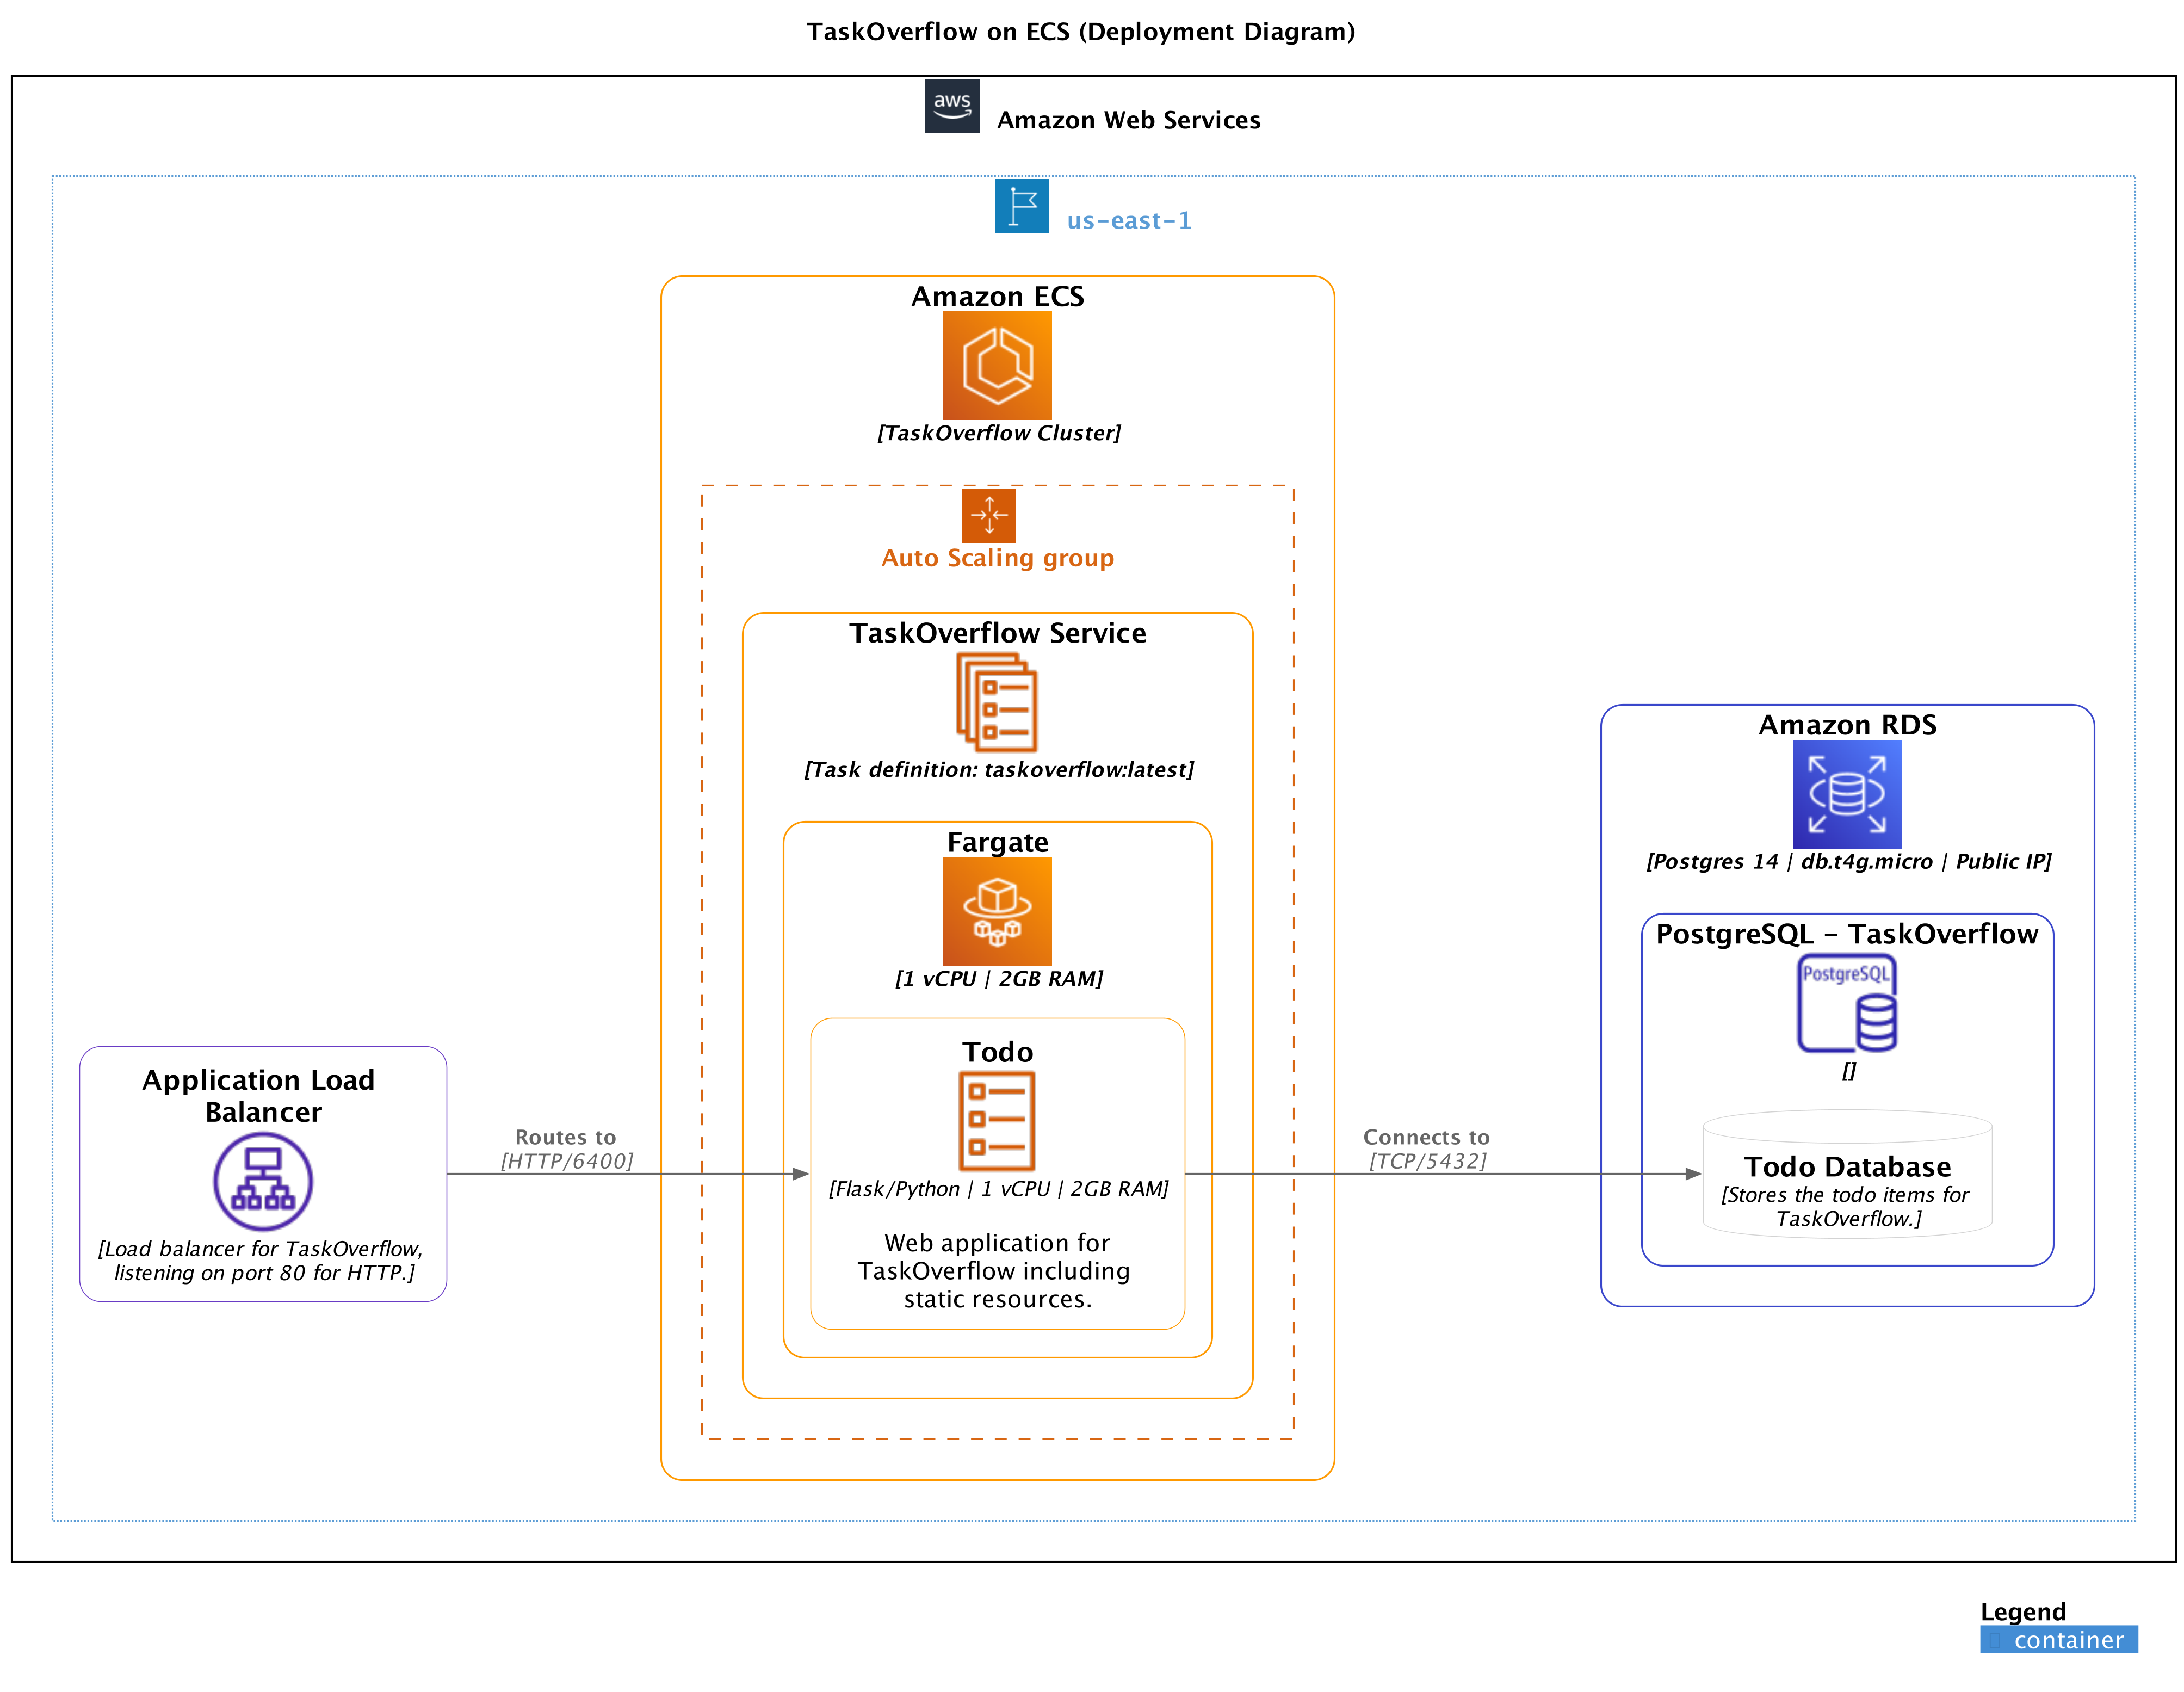
\includegraphics[width=\textwidth]{diagrams/ecsdeployment}
\end{figure}

Last week when we setup the ECS service we noticed that we couldnt get a endpoint cause the instance would only be provisioned after our terraform had run. This is because it is already a dynamic service and it wants a load balancer to service its traffic. To get started we need to create a target group which is on the internal side of the load balancer and defines where traffic can be routed to. Copy this code into \texttt{lb.tf}.

\begin{figure}[H]
  \begin{center}
    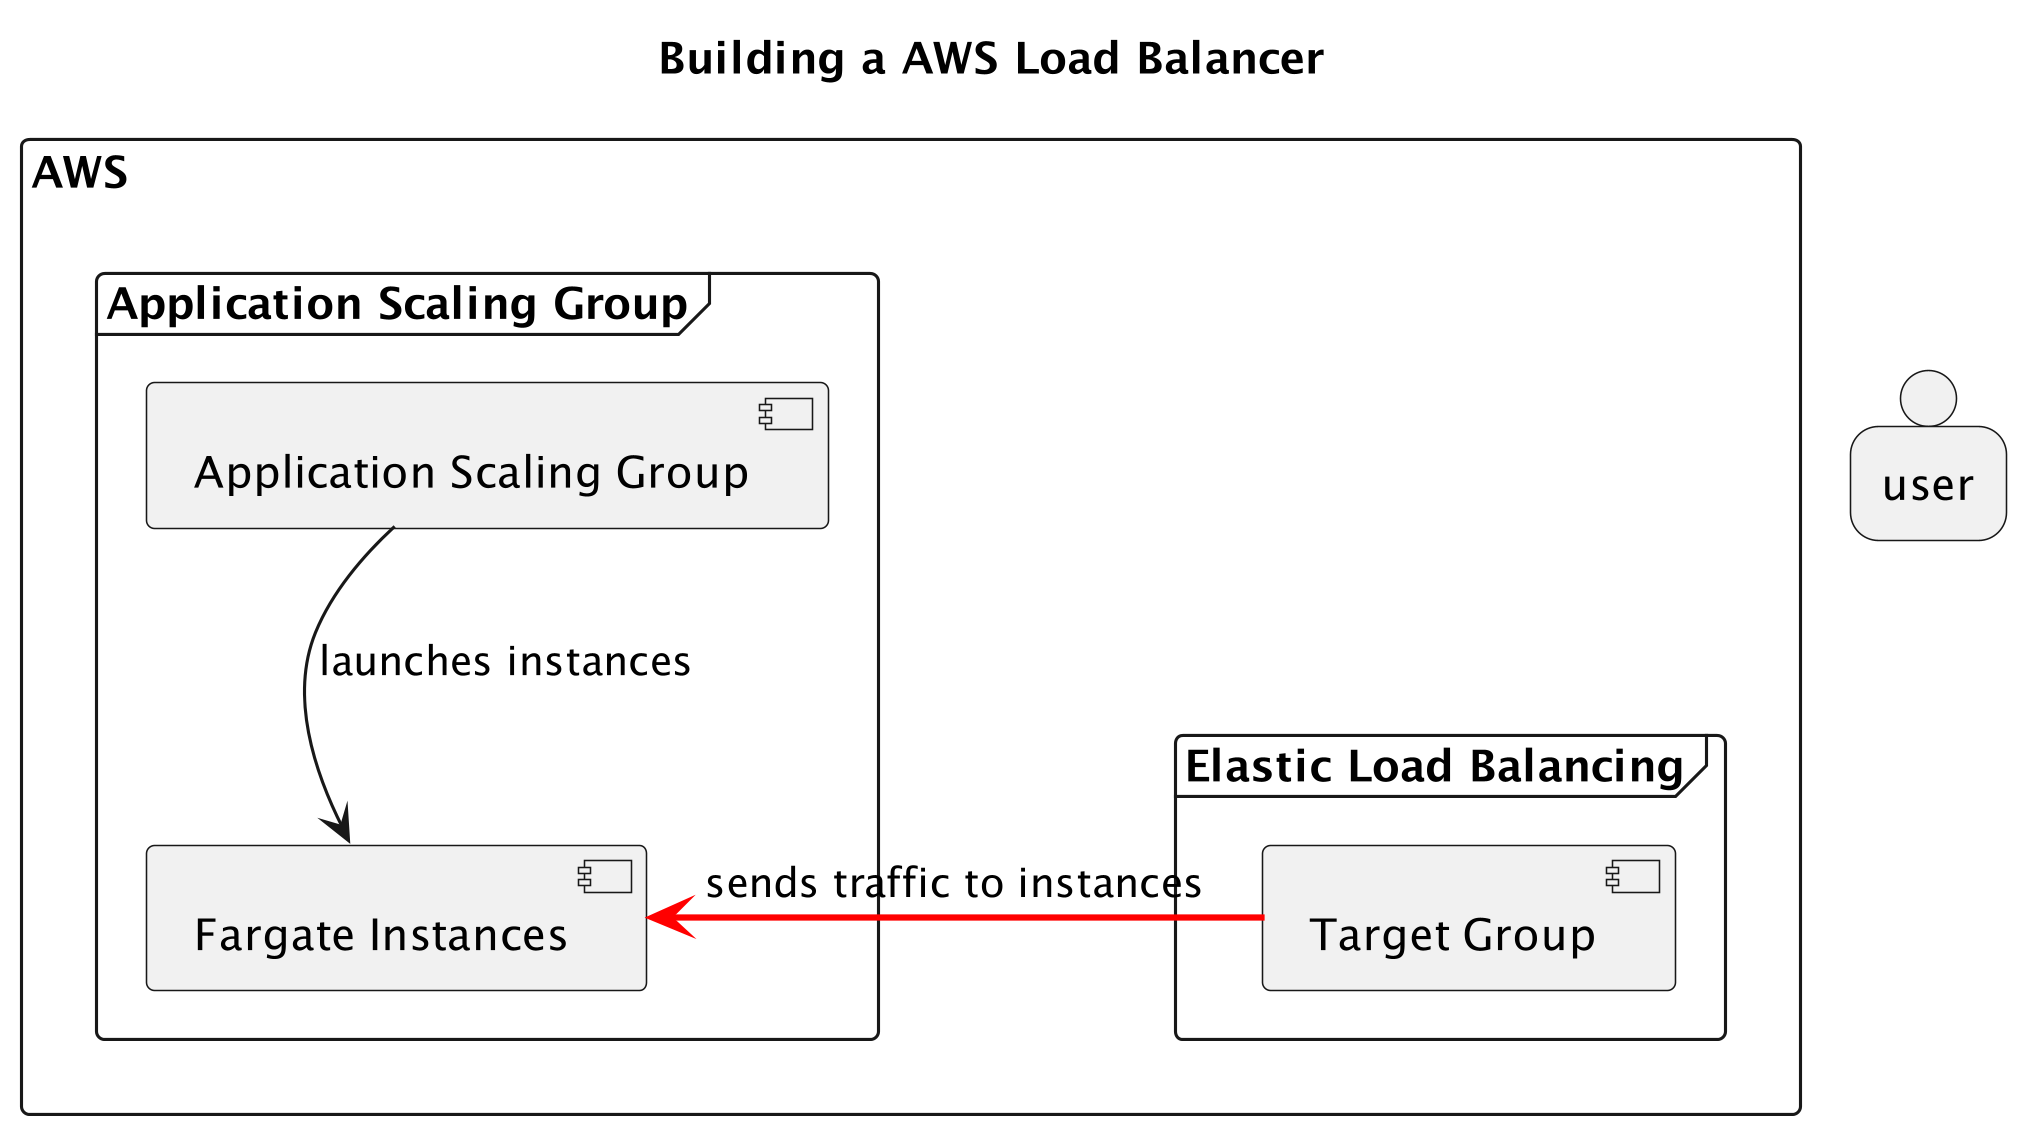
\includegraphics[scale=0.2]{diagrams/lb2fargate}
  \end{center}
\end{figure}

\begin{code}[language=terraform,numbers=none,keepspaces=true]{lb.tf}
resource "aws_lb_target_group" "todo" {
  name          = "todo"
  port          = 6400
  protocol      = "HTTP"
  vpc_id        = aws_security_group.todo.vpc_id
  target_type   = "ip"

  health_check {
    path                = "/api/v1/health"
    port                = "6400"
    protocol            = "HTTP"
    healthy_threshold   = 2
    unhealthy_threshold = 2
    timeout             = 5
    interval            = 10
  }
}
\end{code}

Now that we have the target group we can add it to the ECS service. Copy this code into \texttt{ecs.tf} inside the service block.

\begin{code}[language=terraform,numbers=none,keepspaces=true]{ecs.tf}
  load_balancer {
    target_group_arn = aws_lb_target_group.todo.arn
    container_name   = "todo"
    container_port   = 6400
  }
\end{code}

With the internal side of the load balancer done we can create it and a firewall for the external side. This firewall allows us to restrict what traffic will be allowed to flow through the load balancer. Copy this code into \texttt{lb.tf}.

\begin{figure}[H]
  \begin{center}
    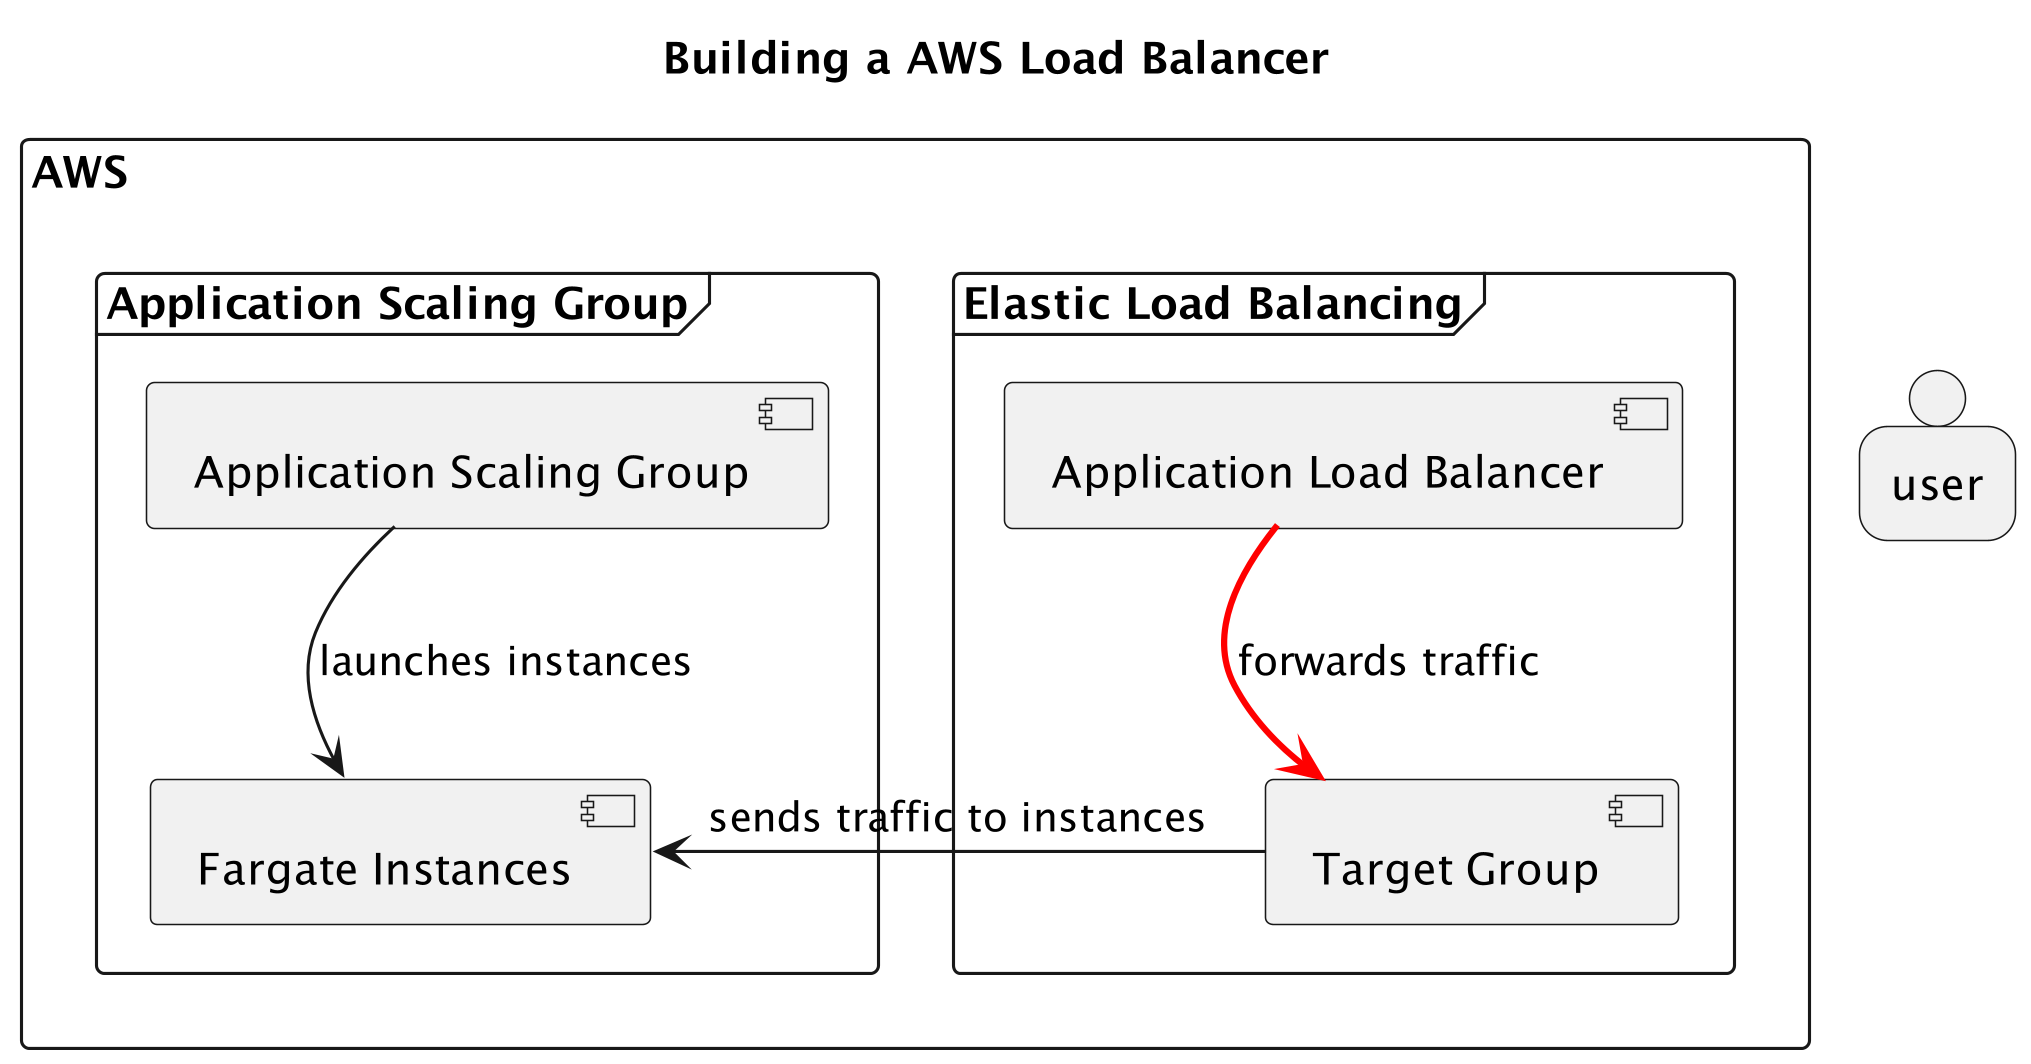
\includegraphics[scale=0.2]{diagrams/lb3fargate}
  \end{center}
\end{figure}

\begin{code}[language=terraform,numbers=none,keepspaces=true]{lb.tf}
resource "aws_lb" "taskoverflow" {
  name               = "taskoverflow"
  internal           = false
  load_balancer_type = "application"
  subnets            = data.aws_subnets.private.ids
  security_groups    = [aws_security_group.taskoverflow.id]
}

resource "aws_security_group" "taskoverflow" {
  name        = "taskoverflow"
  description = "TaskOverflow Security Group"

  ingress {
    from_port     = 80
    to_port       = 80
    protocol      = "tcp"
    cidr_blocks   = ["0.0.0.0/0"]
  }

  egress {
    from_port     = 0
    to_port       = 0
    protocol      = "-1"
    cidr_blocks   = ["0.0.0.0/0"]
  }
}
\end{code}

Now over to the external side of the load balancer we need to create a listener which is the entry point for the load balancer. Copy this code into \texttt{lb.tf}.

\begin{figure}[H]
  \begin{center}
    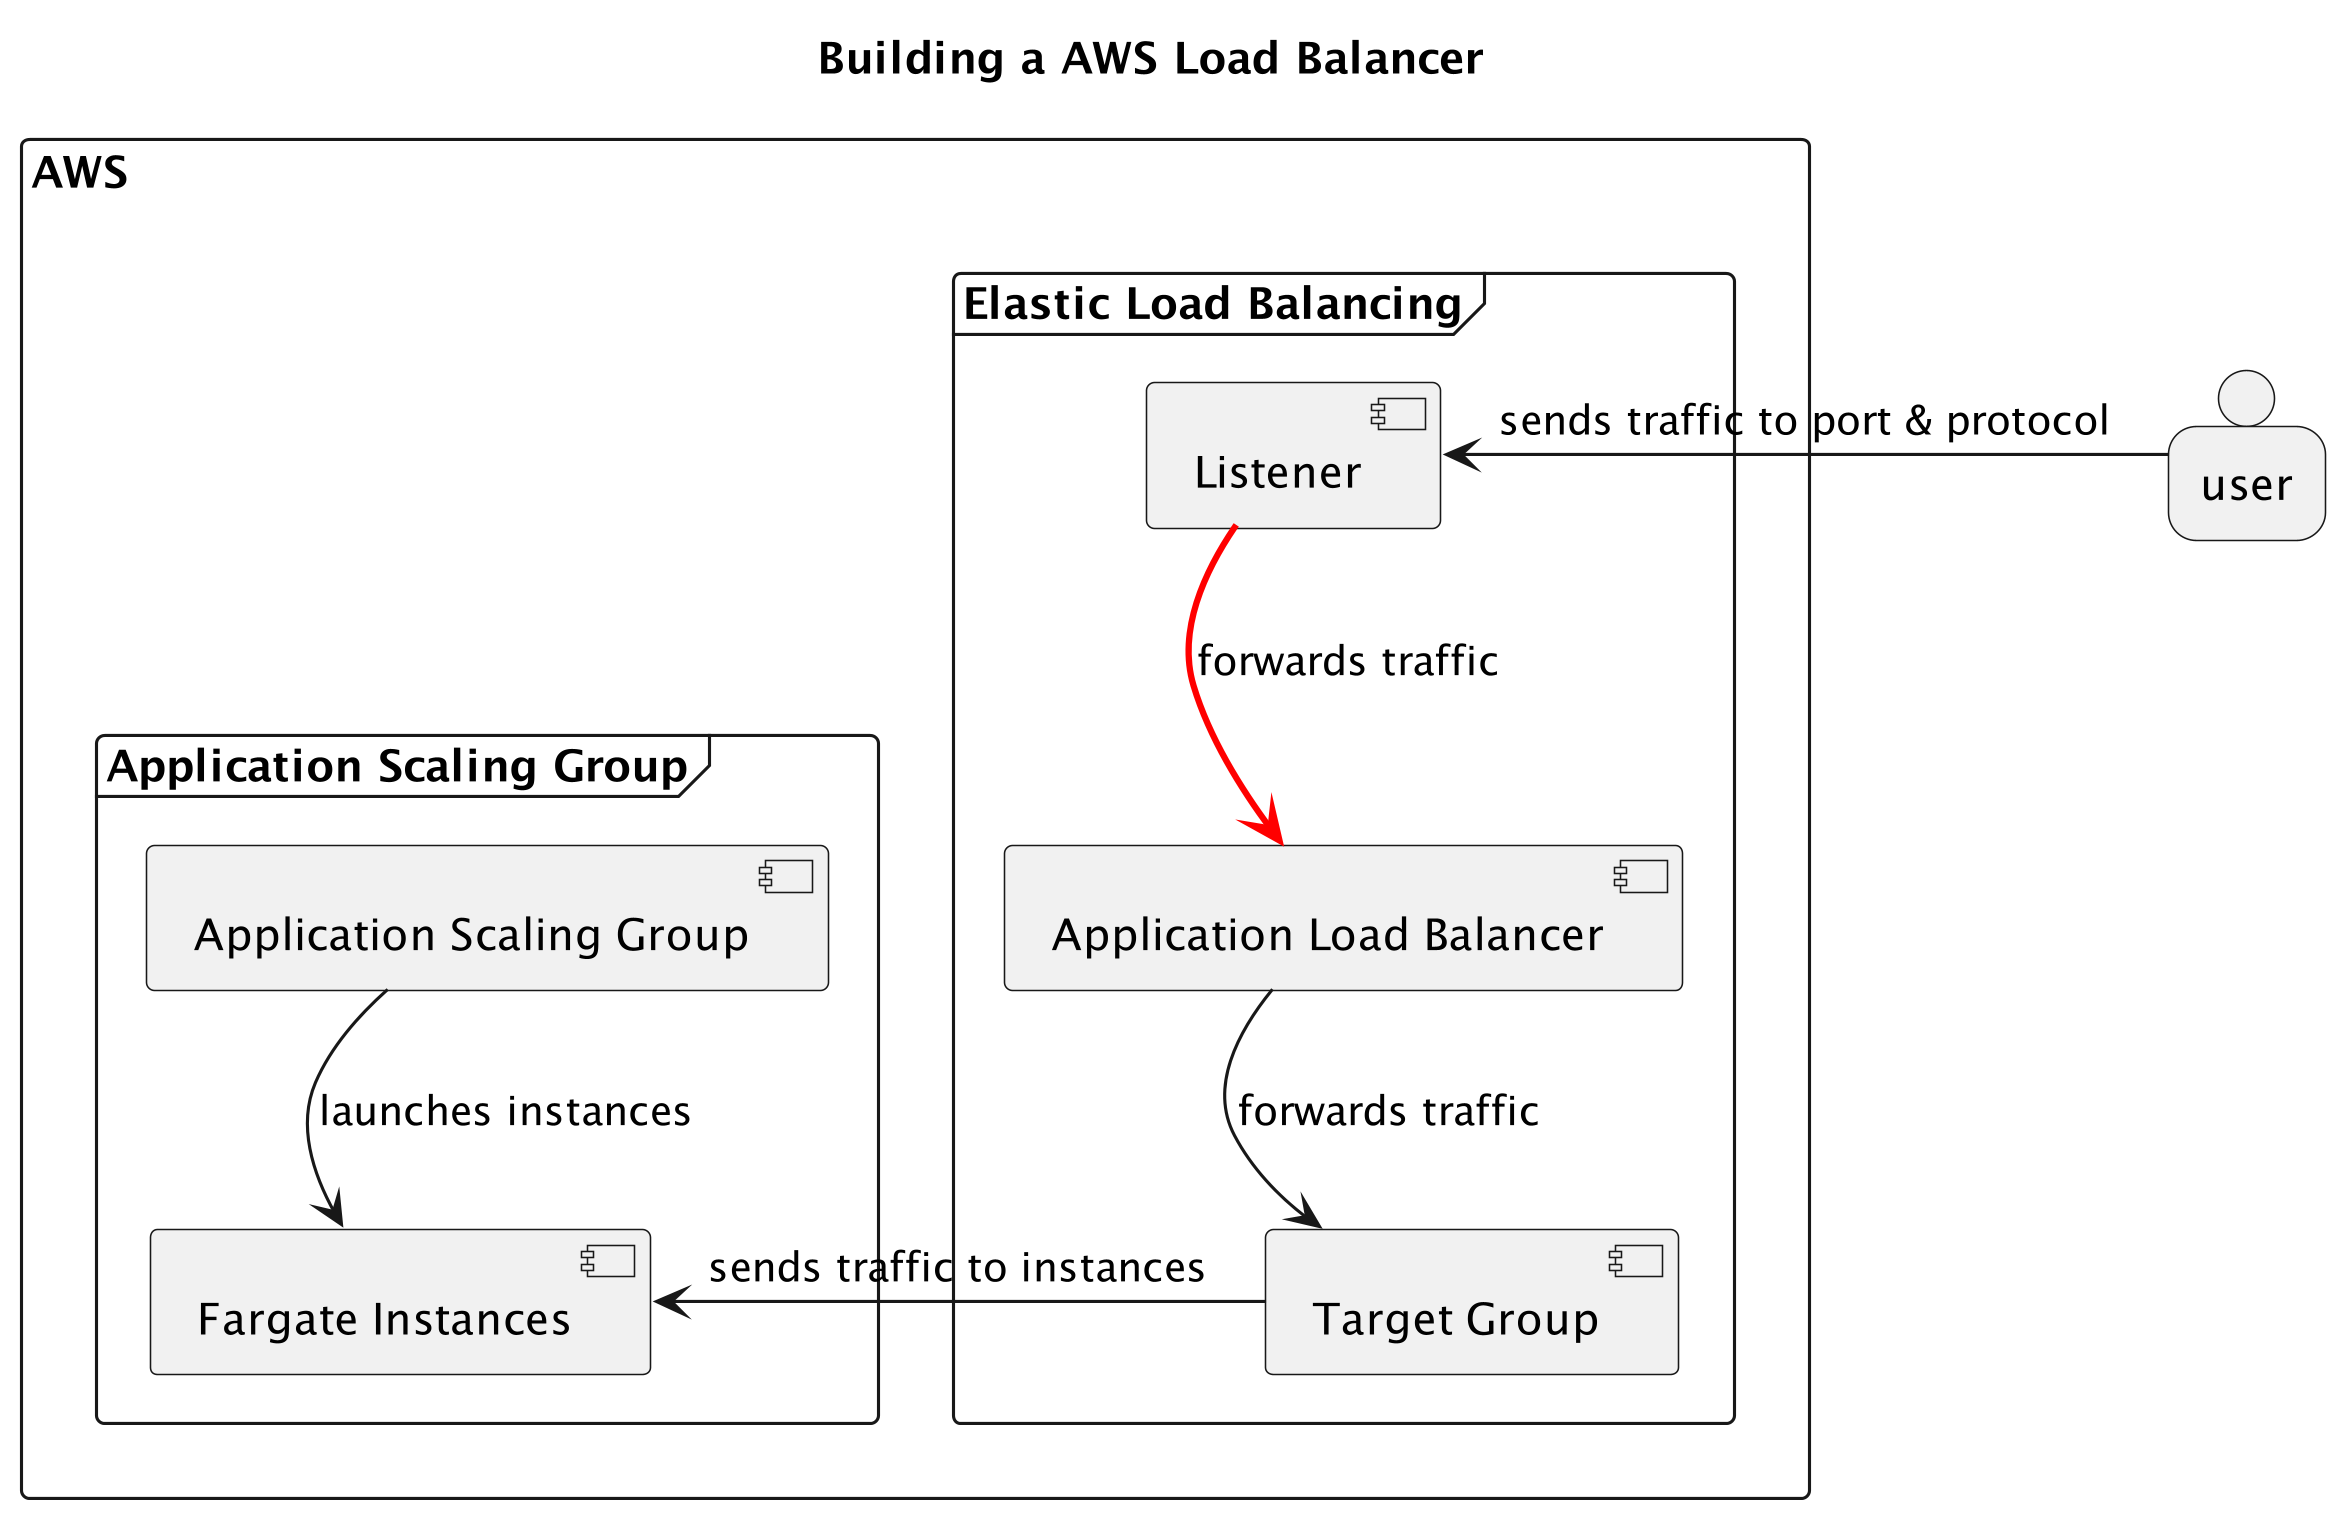
\includegraphics[scale=0.2]{diagrams/lb4fargate}
  \end{center}
\end{figure}

\begin{code}[language=terraform,numbers=none,keepspaces=true]{lb.tf}
resource "aws_lb_listener" "todo" {
  load_balancer_arn   = aws_lb.taskoverflow.arn
  port                = "80"
  protocol            = "HTTP"

  default_action {
    type              = "forward"
    target_group_arn  = aws_lb_target_group.todo.arn
  }
}
\end{code}

If we deployed now we would have completed the deployment diagram above. However we want to add some autoscaling to our service so that it can scale up and down based on the load. Copy this code into \texttt{autoscaling.tf}.

\begin{code}[language=terraform,numbers=none,keepspaces=true]{autoscaling.tf}
resource "aws_appautoscaling_target" "todo" {
  max_capacity        = 4
  min_capacity        = 1
  resource_id         = "service/taskoverflow/taskoverflow"
  scalable_dimension  = "ecs:service:DesiredCount"
  service_namespace   = "ecs"
}


resource "aws_appautoscaling_policy" "todo-cpu" {
  name                = "todo-cpu"
  policy_type         = "TargetTrackingScaling"
  resource_id         = aws_appautoscaling_target.todo.resource_id
  scalable_dimension  = aws_appautoscaling_target.todo.scalable_dimension
  service_namespace   = aws_appautoscaling_target.todo.service_namespace

  target_tracking_scaling_policy_configuration {
    predefined_metric_specification {
      predefined_metric_type  = "ECSServiceAverageCPUUtilization"
    }

    target_value              = 20
  }
}
\end{code}

This auto scaling policy looks at the average CPU utilization of the service and scales up if it is above 20\% and scales down if it is below 20\%. This is a very simple policy but it is a good starting point. We can now deploy our service and see it scale up and down. Continue onto the next section to see how to send our service some load.

\subsection{Producing Load with K6}

We have a service but us visiting it in our web browser is not gonna trigger enough load for our policies to trigger. To do this we are gonna employ the help of a tool called K6 which is a recent addition to the load testing tools. To install K6 visit \url{https://k6.io/docs/get-started/installation/}, this can be installed in the code spaces environment or locally.

We have provided an example K6 file which is a javascript script that creates 1000 to 5000 users to call the list endpoint of our service. Copy this code into a file called \texttt{k6.js}.

\begin{code}[language=javascript,numbers=none,escapechar=!]{k6.js}
import http from 'k6/http';
import { sleep, check } from 'k6';

export const options = {
  stages: [
    { target: 1000, duration: '1m' },
    { target: 5000, duration: '10m' },
  ],
};

export default function () {
  const res = http.get('http://!\colorbox{yellow}{your-loadBalancer-url-here}!/api/v1/todos');
  check(res, { 'status was 200': (r) => r.status == 200 });
  sleep(1);
}
\end{code}

we can then run this file using the following command.

\begin{code}[language=bash,numbers=none,keepspaces=true]{}
>> k6 run k6.js
\end{code}

\begin{code}[language=bash,numbers=none,keepspaces=true]{}
execution: local
  script: load.js
  output: -

scenarios: (100.00%) 1 scenario, 5000 max VUs, 11m30s max duration (incl. graceful stop):
        * default: Up to 5000 looping VUs for 11m0s over 2 stages (gracefulRampDown: 30s, gracefulStop: 30s)


running (00m05.4s), 0091/5000 VUs, 140 complete and 0 interrupted iterations
default   [--------------------------------------] 0091/5000 VUs  00m05.4s/11m00.0s

\end{code}

\subsubsection{EC2 Auto Scaling}

\todo{Show where in AWS they can see the scaling events for EC2}

\begin{figure}[H]
  \begin{center}
    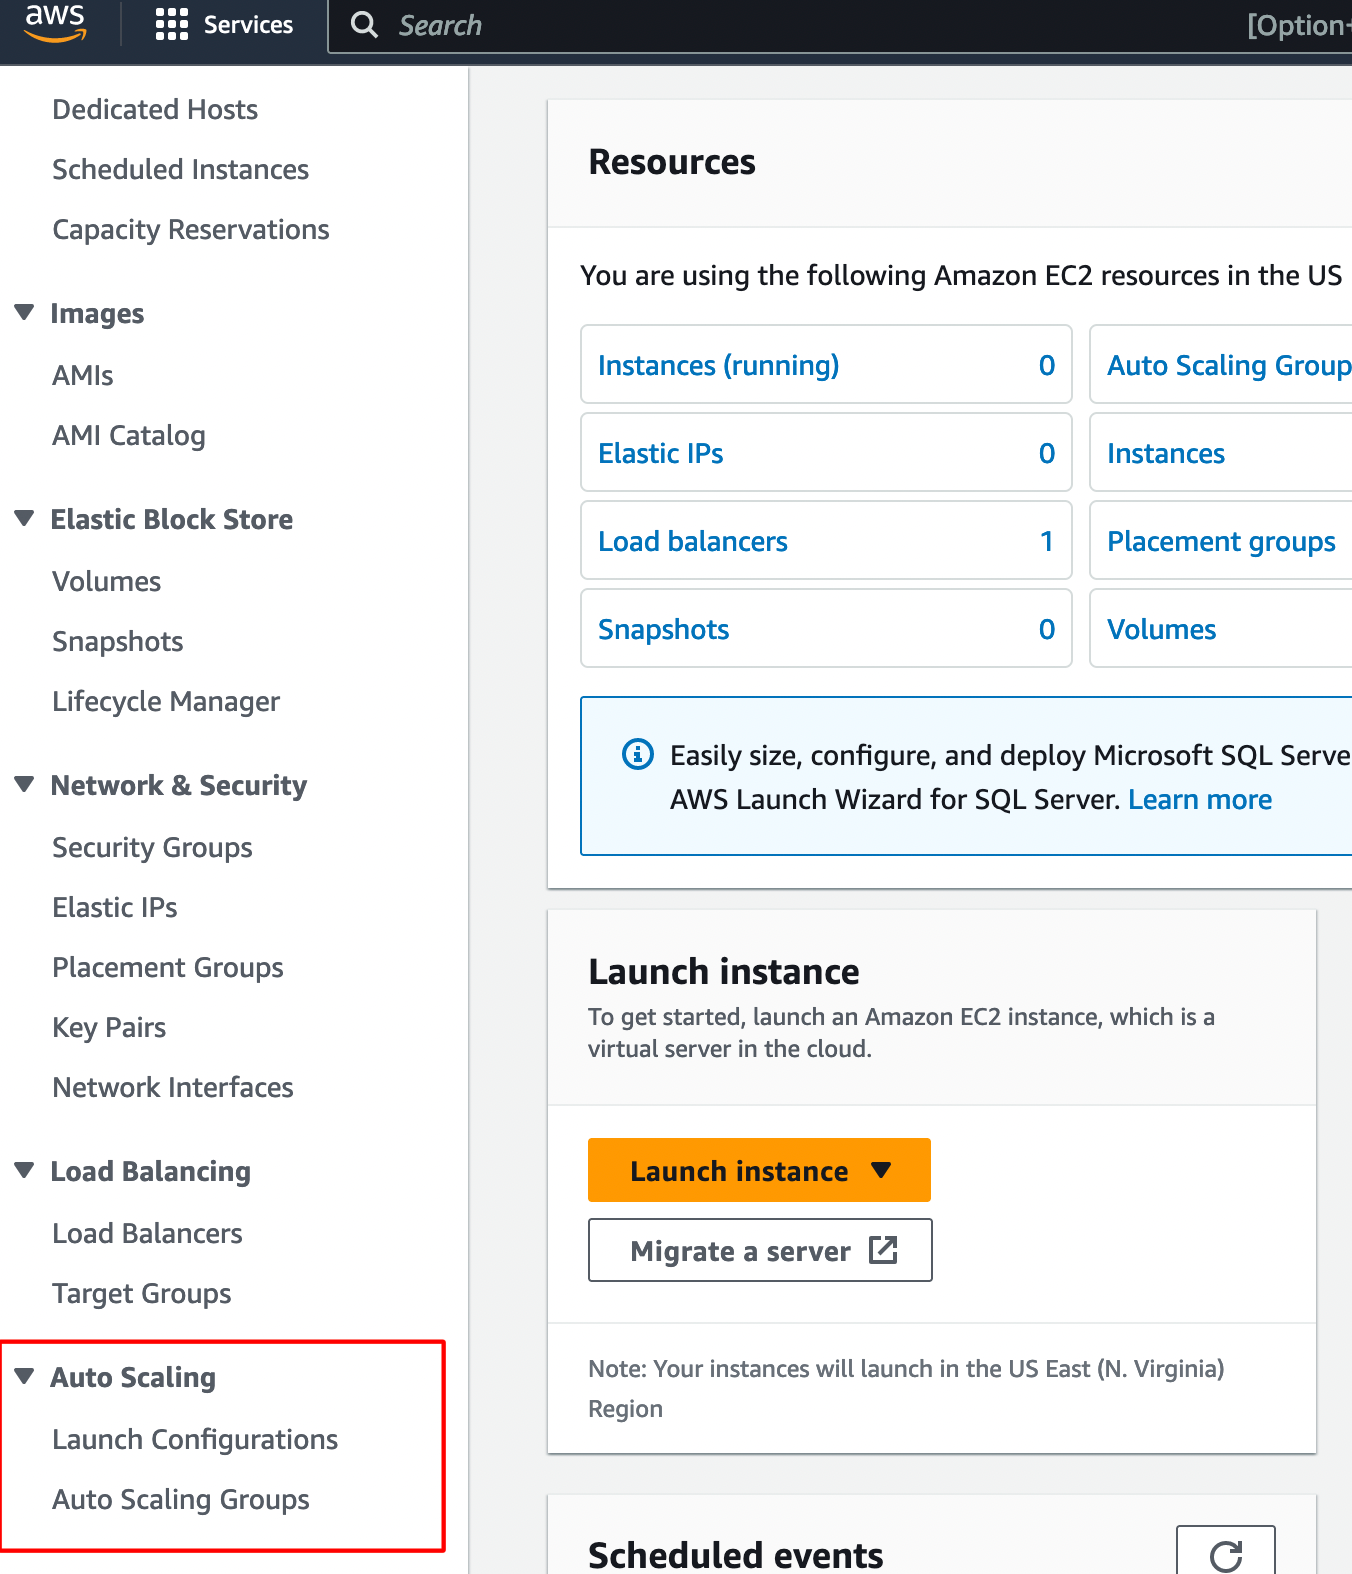
\includegraphics[scale=0.5]{images/ec2_1}
  \end{center}
\end{figure}

\begin{figure}[H]
  \begin{center}
    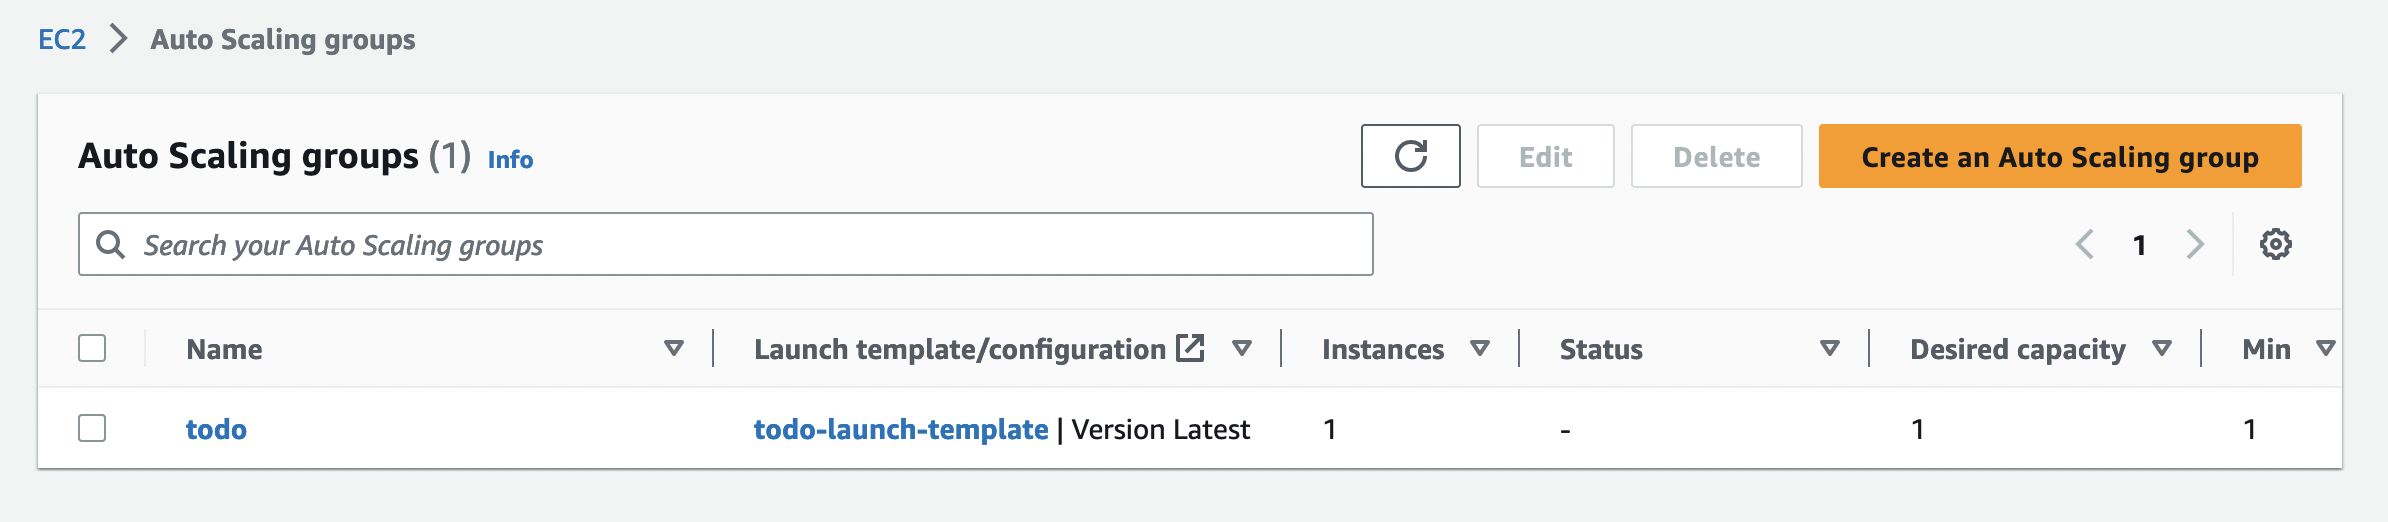
\includegraphics[width=\textwidth]{images/ec2_3}
  \end{center}
\end{figure}

\begin{figure}[H]
  \begin{center}
    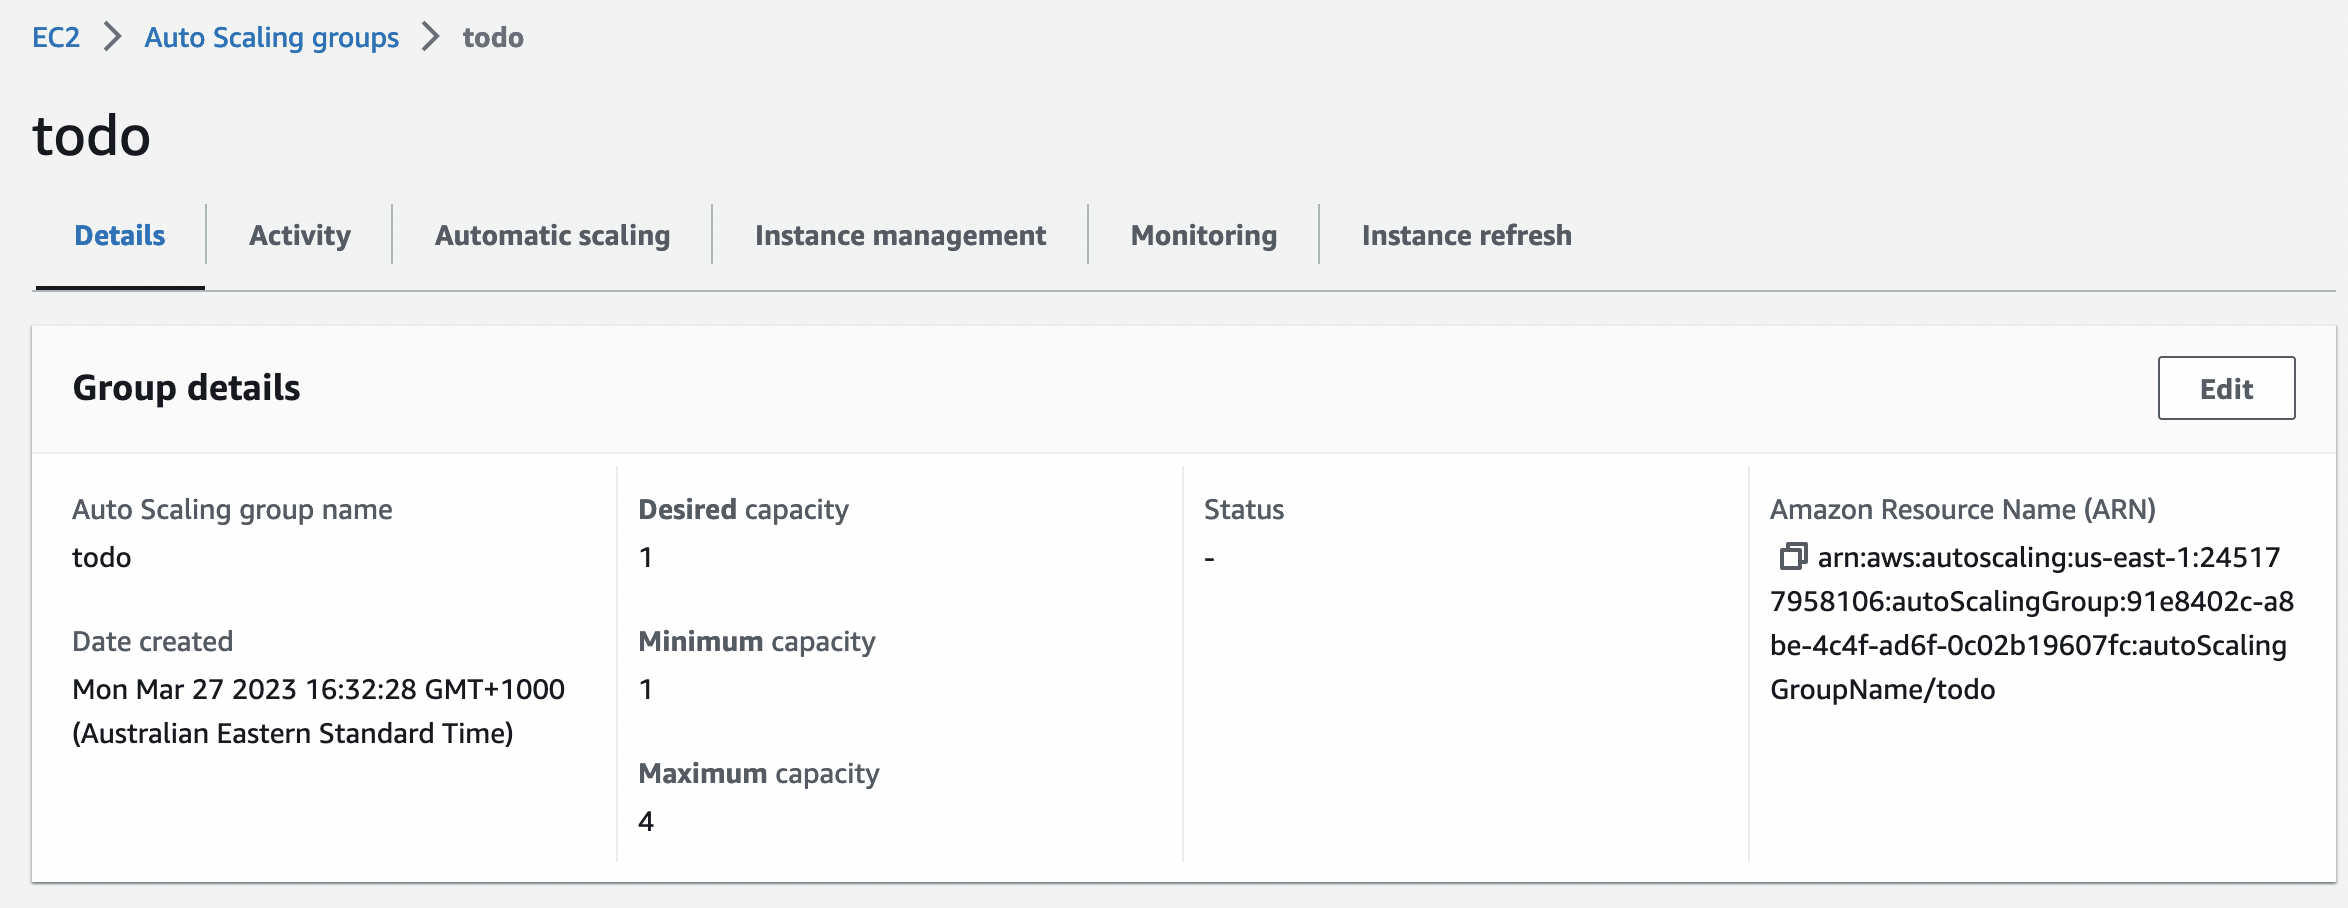
\includegraphics[width=\textwidth]{images/ec2_4}
  \end{center}
\end{figure}

\begin{figure}[H]
  \begin{center}
    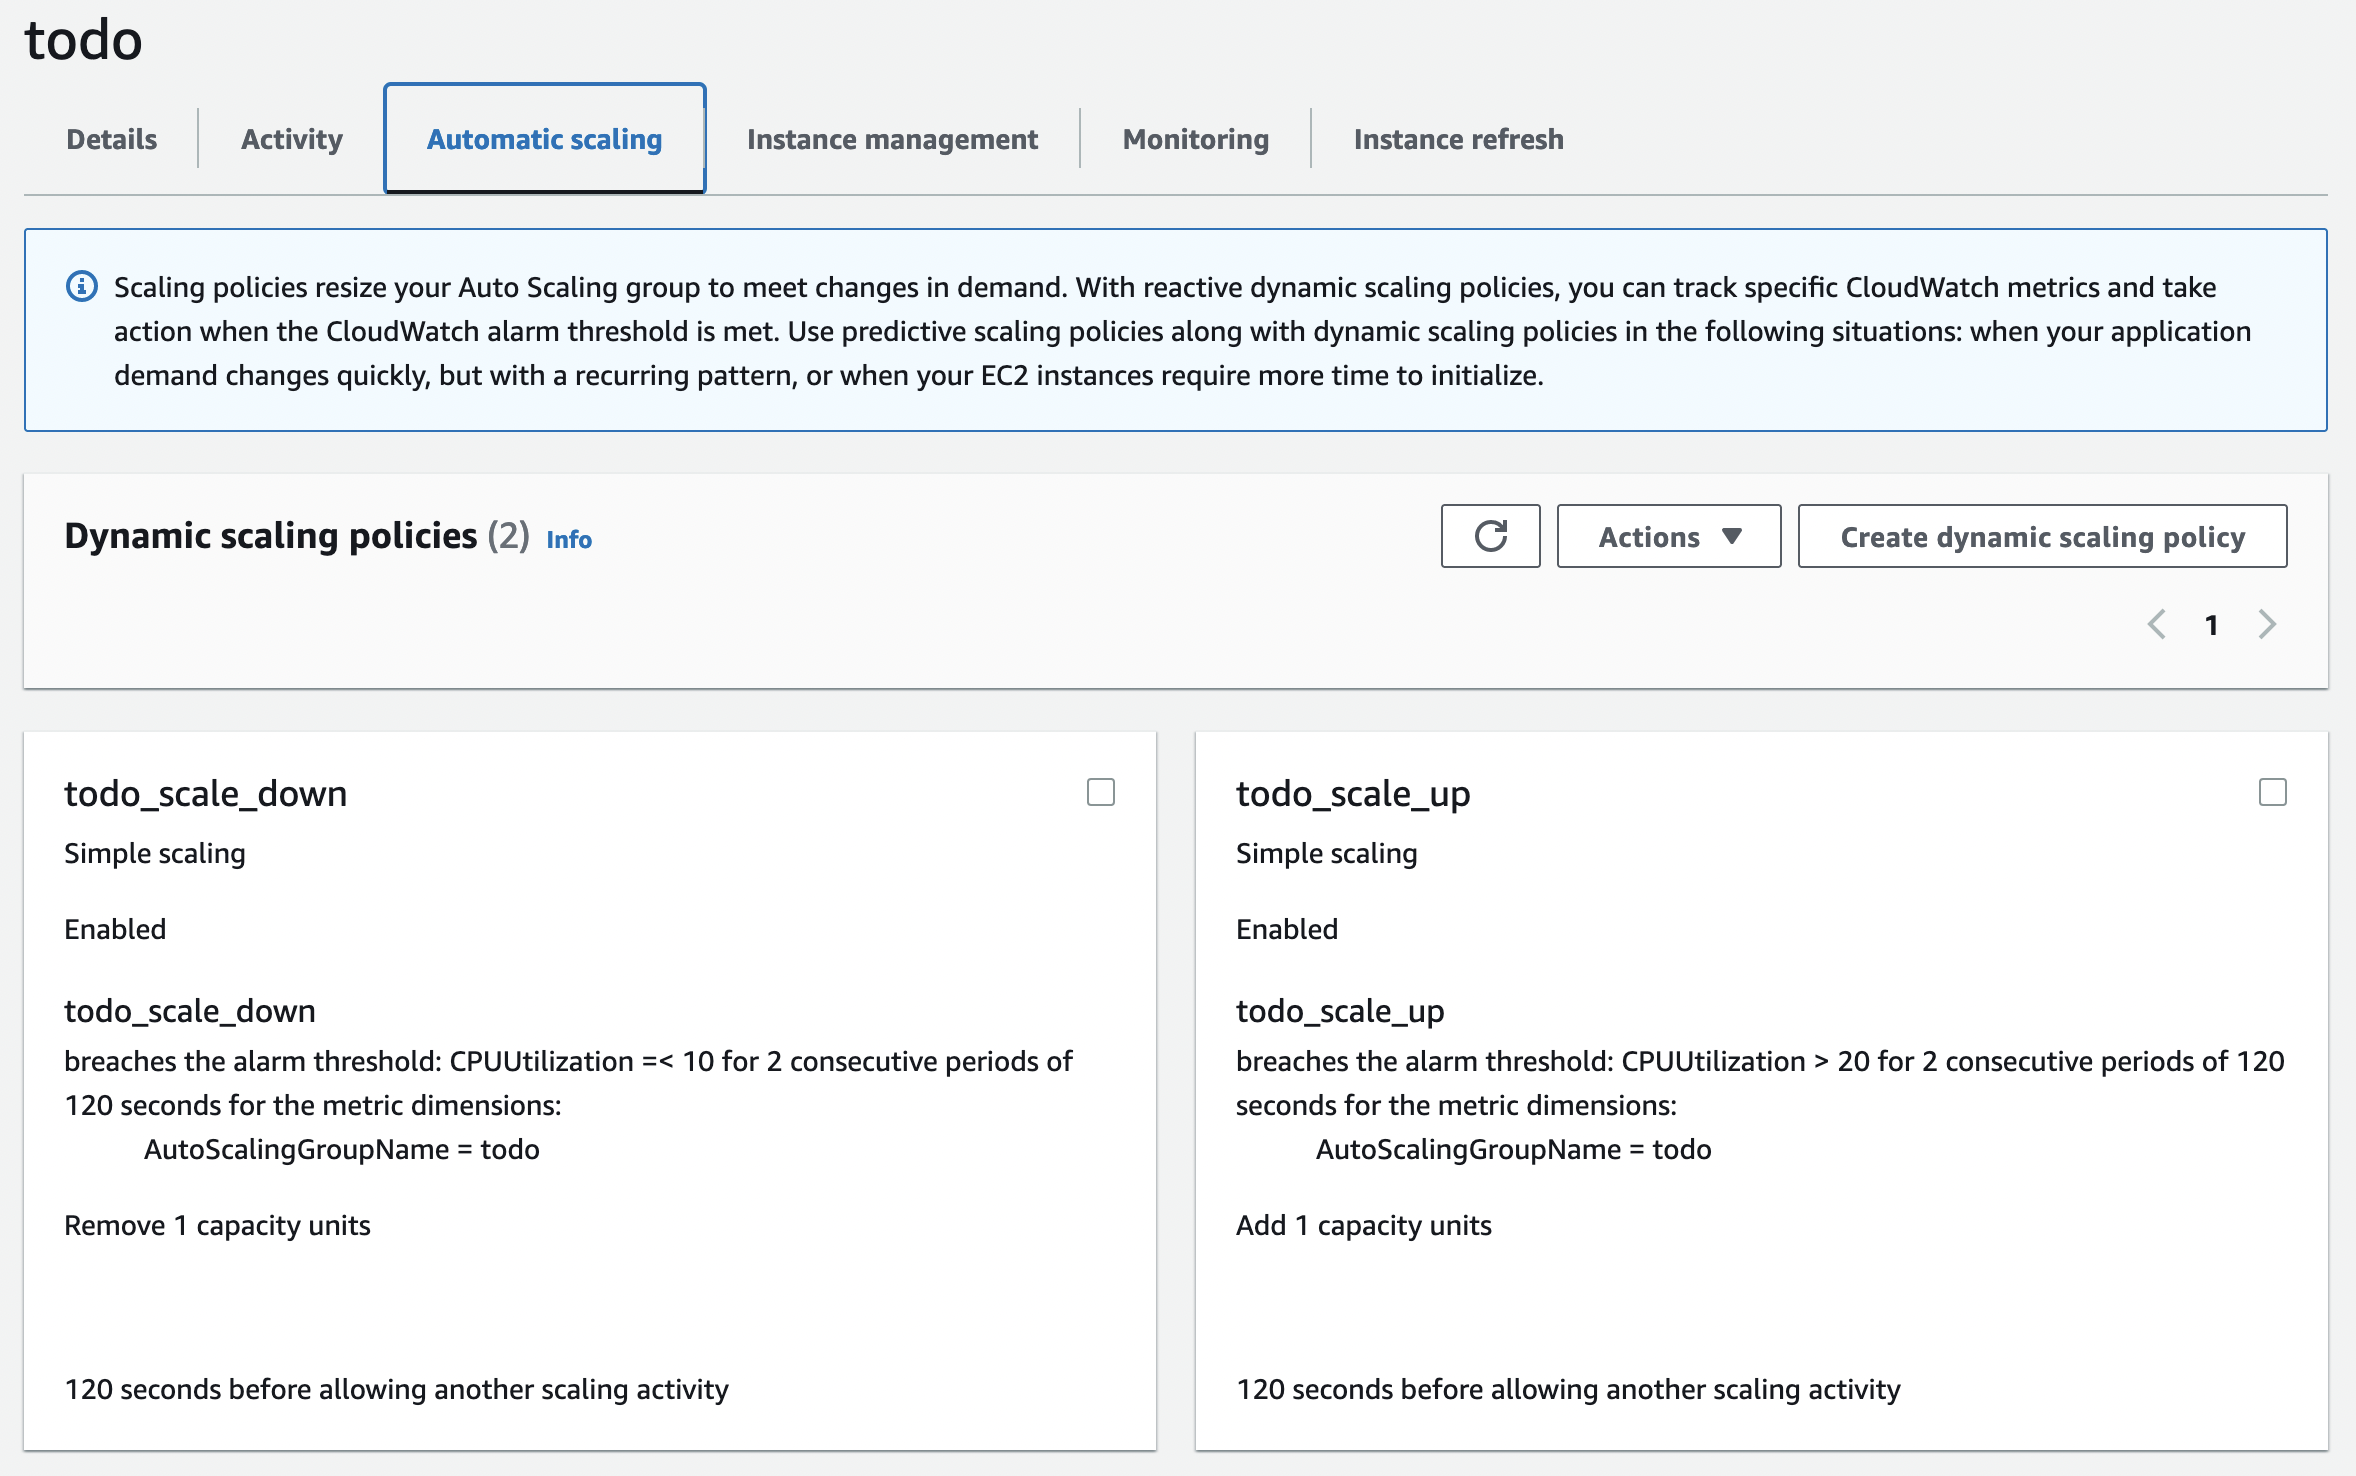
\includegraphics[width=\textwidth]{images/ec2_5}
  \end{center}
\end{figure}

\begin{figure}[H]
  \begin{center}
    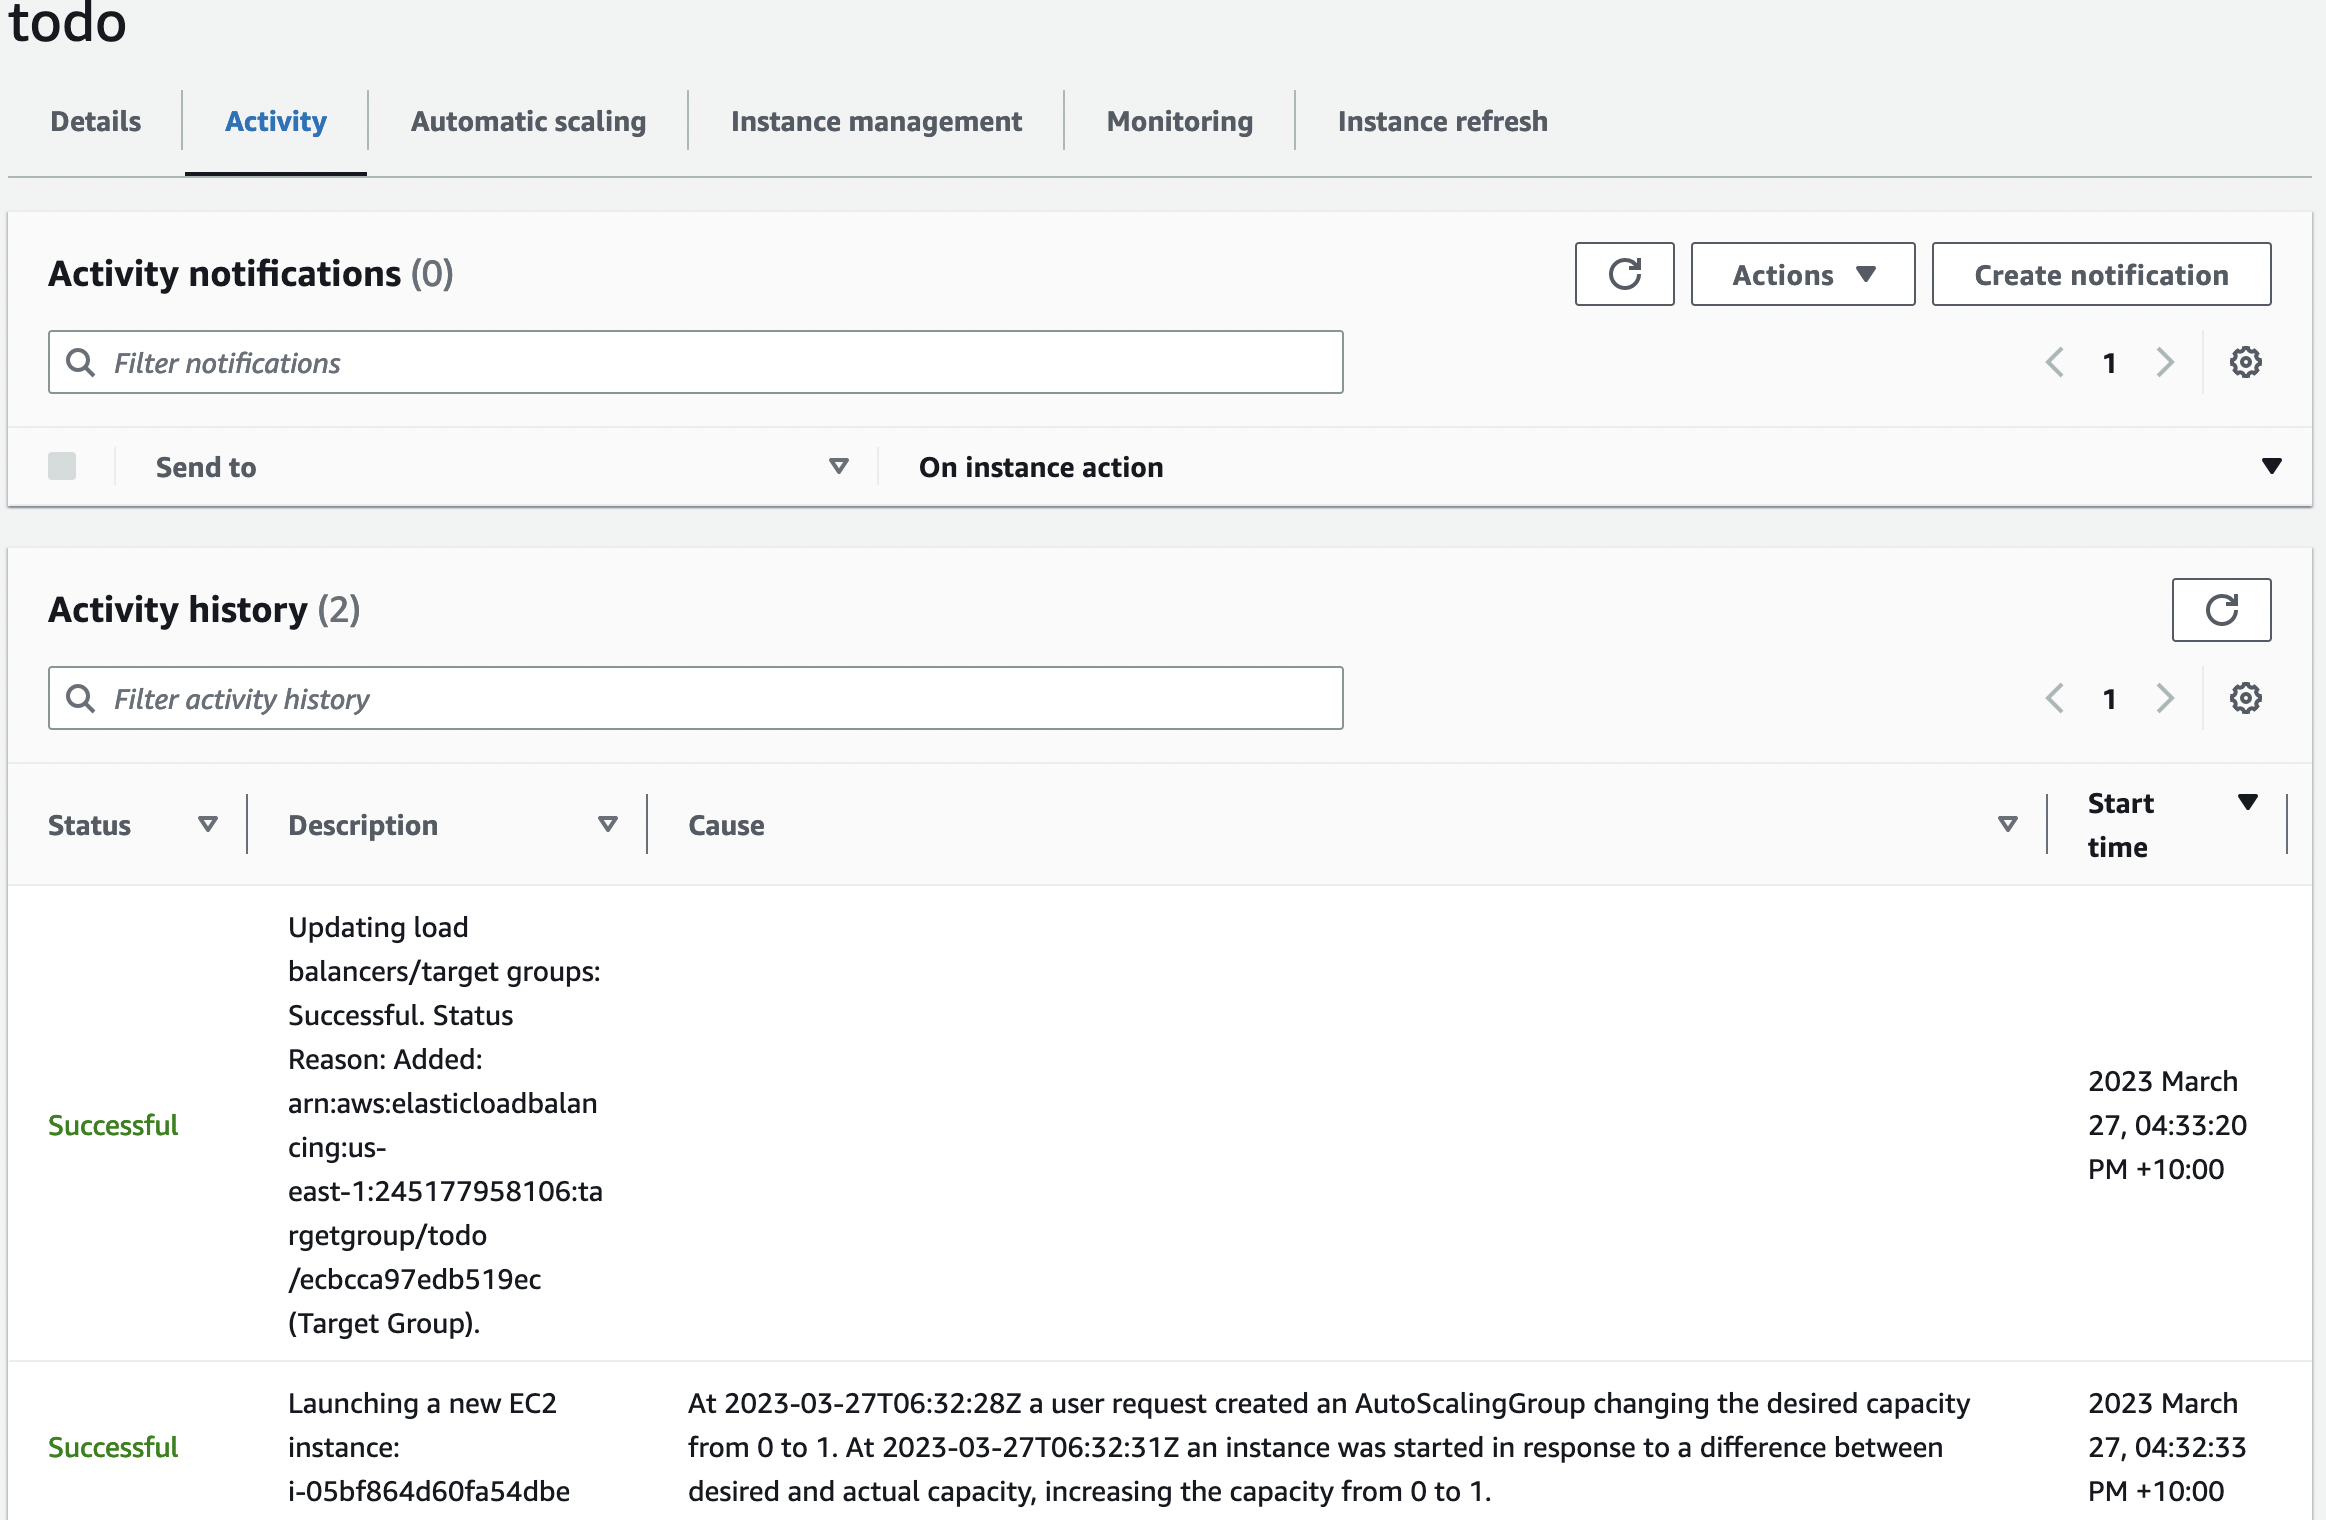
\includegraphics[width=\textwidth]{images/ec2_6}
  \end{center}
\end{figure}

\begin{figure}[H]
  \begin{center}
    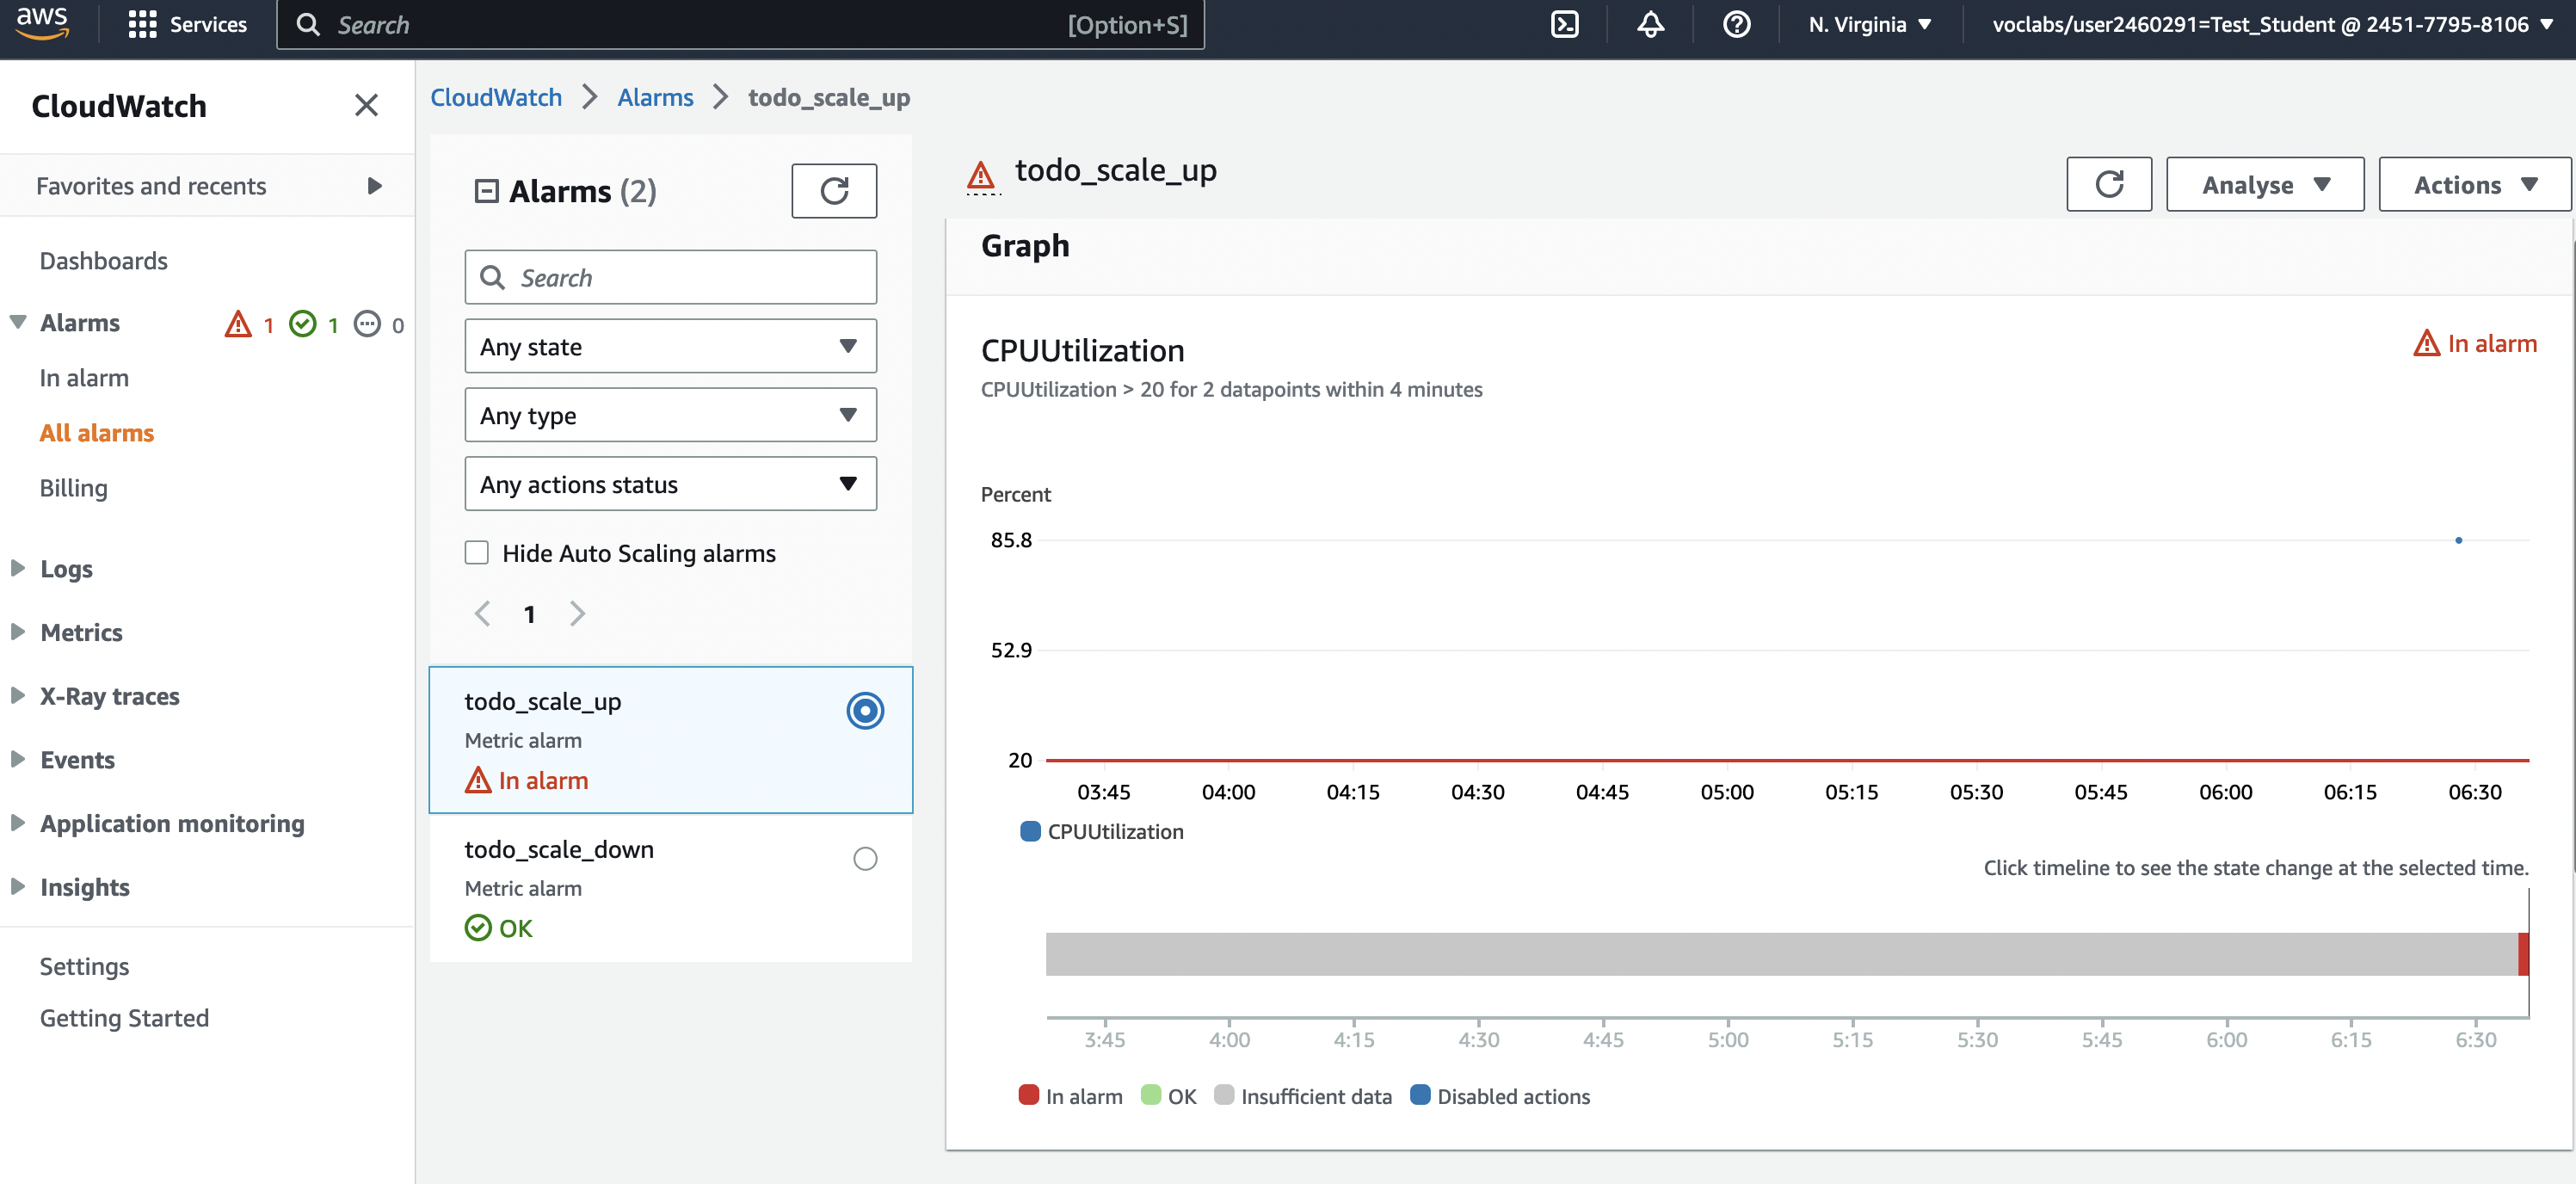
\includegraphics[width=\textwidth]{images/ec2_7}
  \end{center}
\end{figure}

\subsubsection{ECS Auto Scaling}

\todo{Show where in AWS they can see the scaling events for ECS}

\begin{figure}[H]
  \begin{center}
    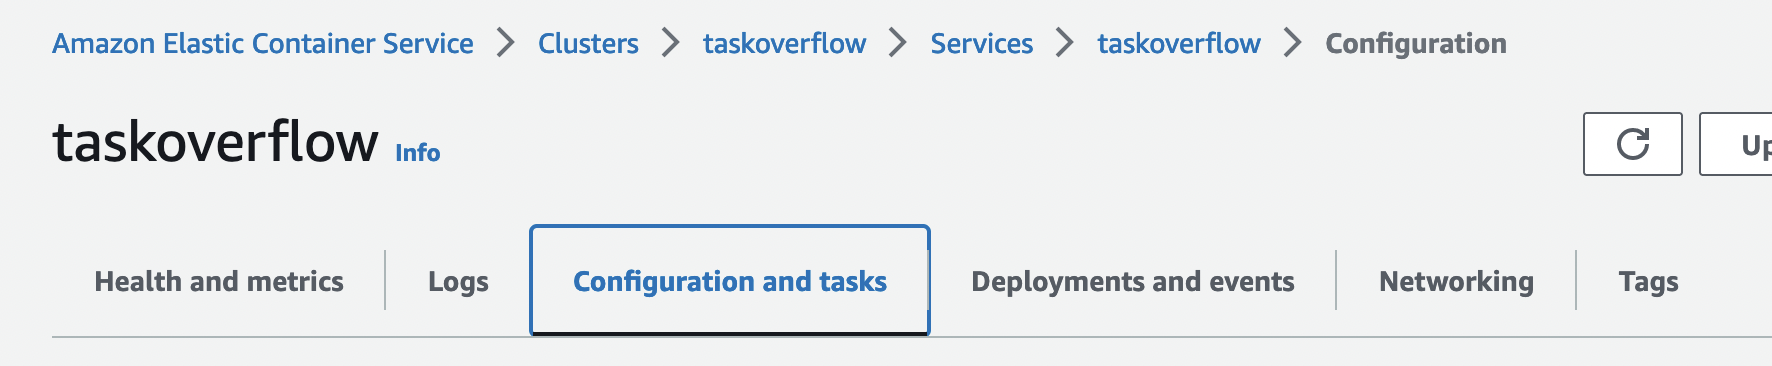
\includegraphics[width=\textwidth]{images/ecs1}
  \end{center}
\end{figure}

\begin{figure}[H]
  \begin{center}
    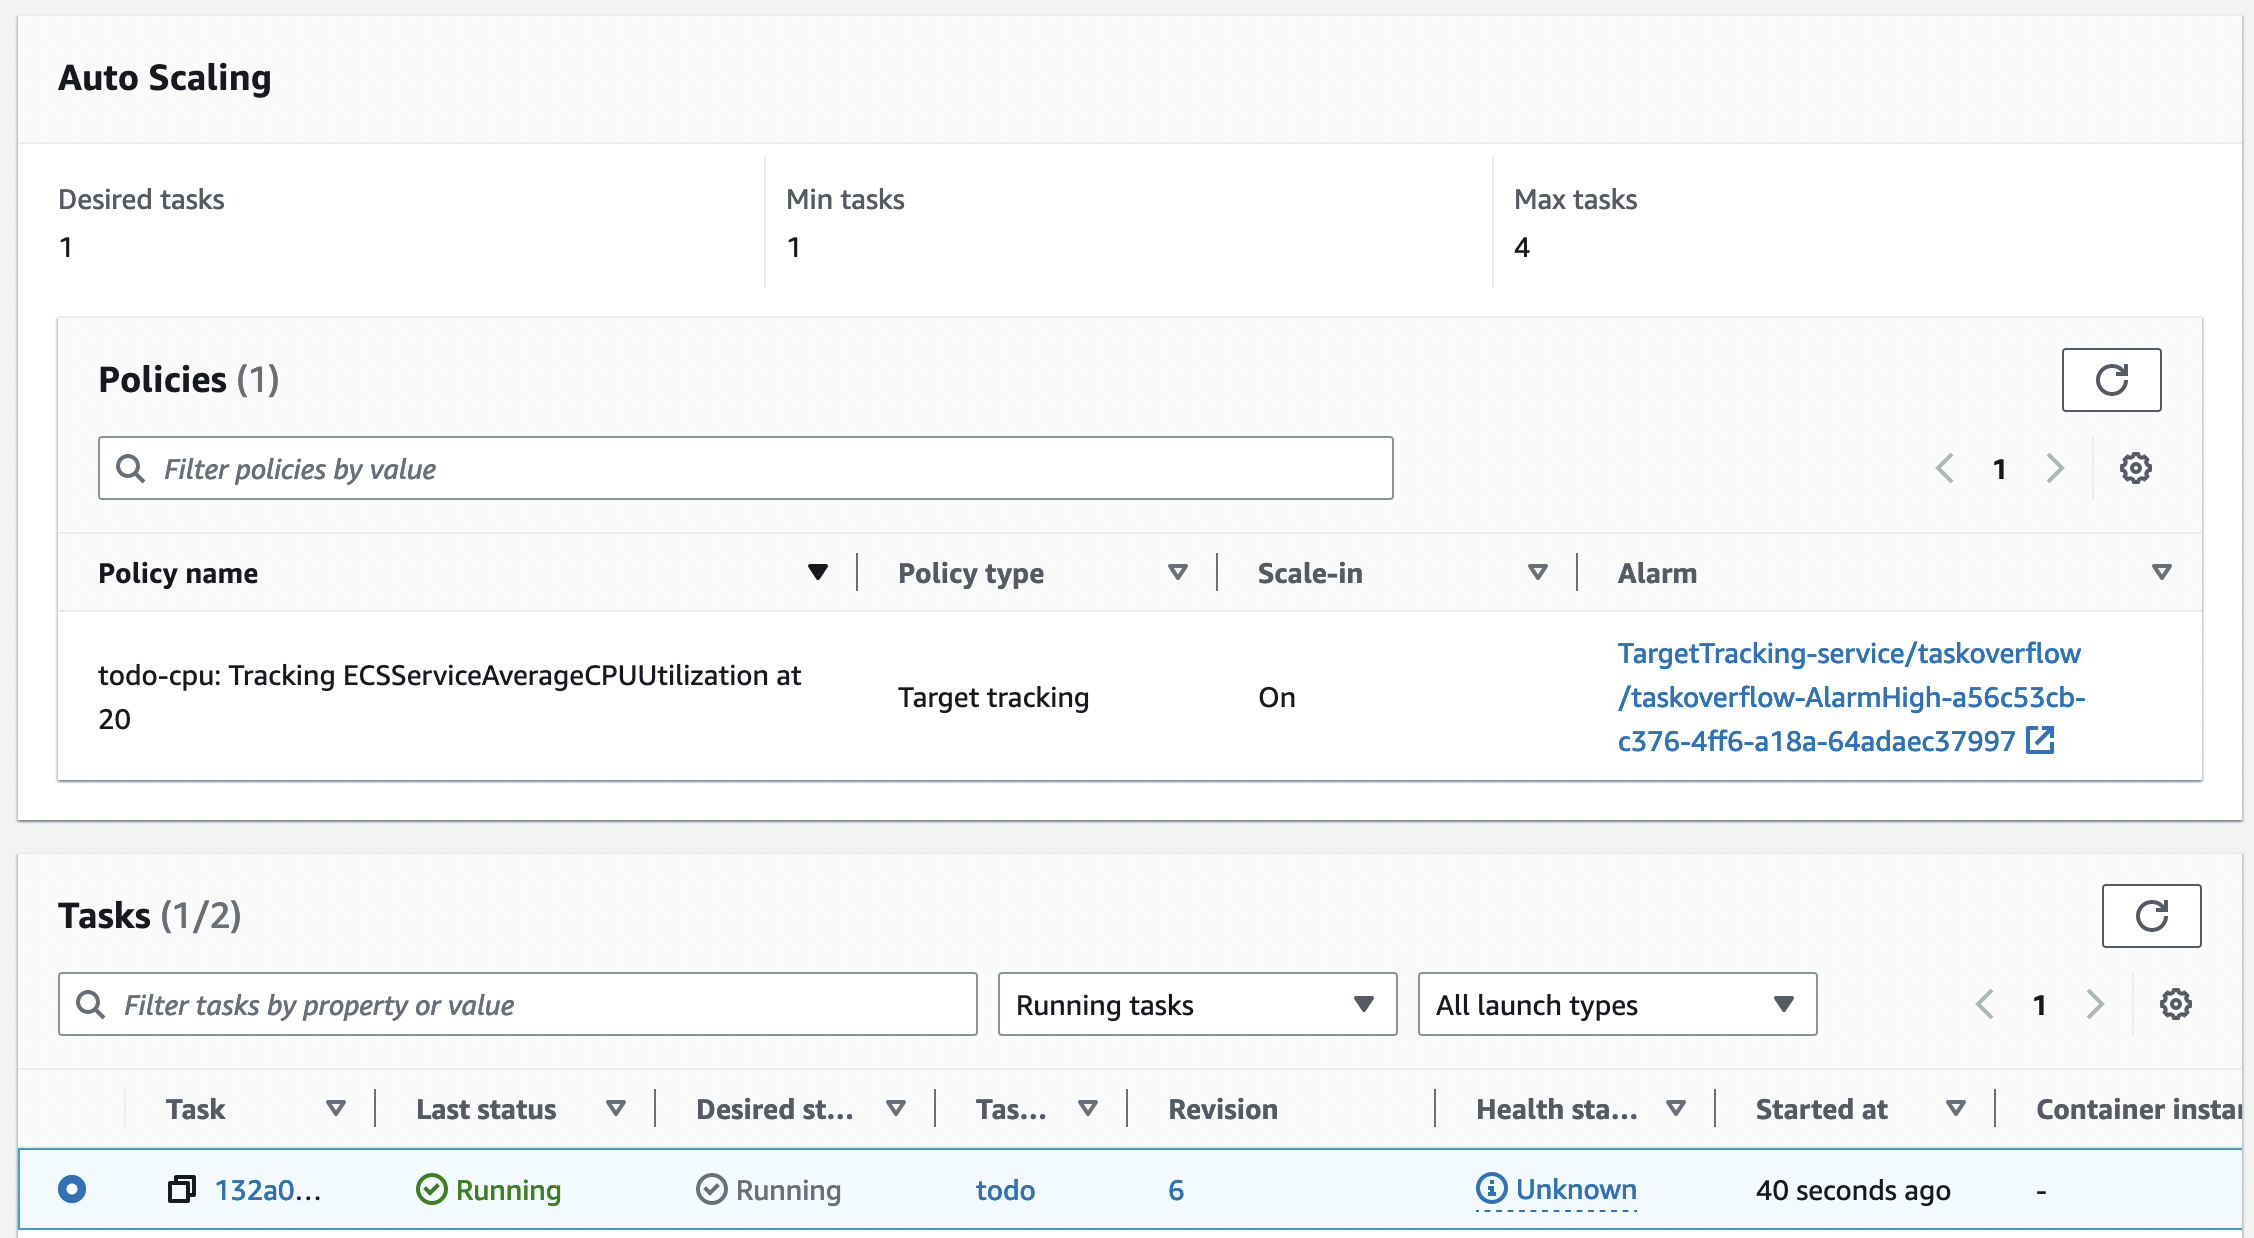
\includegraphics[width=\textwidth]{images/ecs2}
  \end{center}
\end{figure}

\begin{figure}[H]
  \begin{center}
    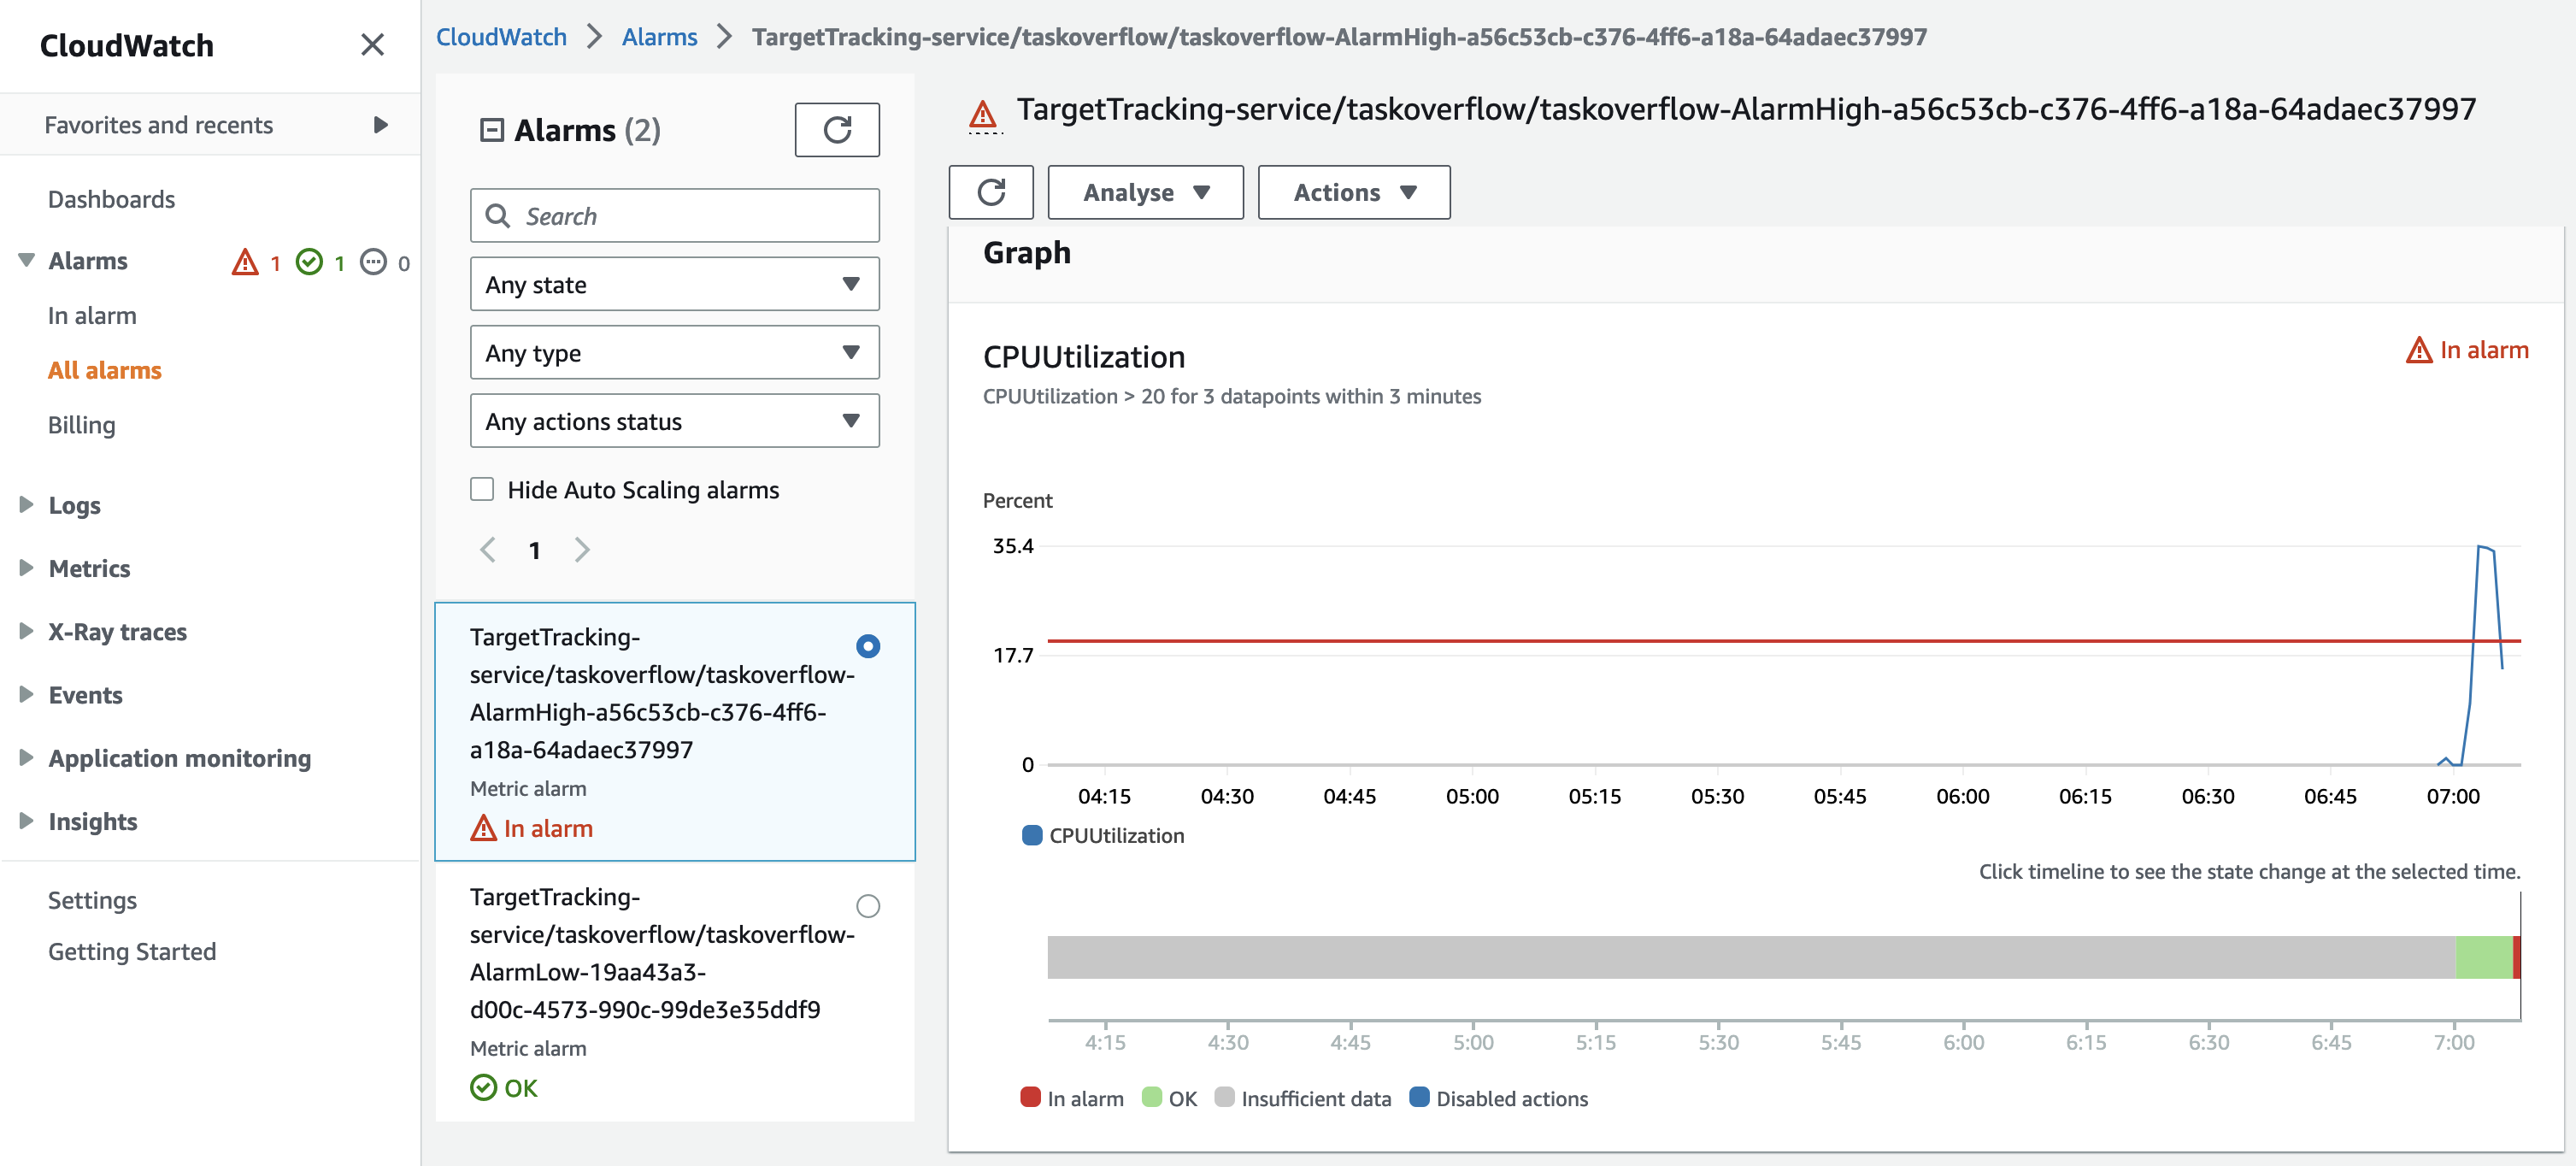
\includegraphics[width=\textwidth]{images/ecs3}
  \end{center}
\end{figure}

\bibliographystyle{ieeetr}
\bibliography{books,ours}

\end{document}
